%%=============================================================================
%% LaTeX sjabloon voor bachelorproef, HoGent Bedrijf en Organisatie
%% Opleiding Toegepaste Informatica
%%=============================================================================

\documentclass[fleqn,a4paper,12pt]{book}

%%=============================================================================
%% LaTeX sjabloon voor de bachelorproef, HoGent Bedrijf en Organisatie
%% Opleiding toegepaste informatica
%%
%% Structuur en algemene vormgeving. Meestal hoef je hier niets te wijzigen.
%%
%% Vormgeving gebaseerd op "The Legrand Orange Book", version 2.0 (9/2/15)
%% door Mathias Legrand (legrand.mathias@gmail.com) met aanpassingen door
%% Vel (vel@latextemplates.com). Het oorspronkelijke template is te vinden op
%% http://www.LaTeXTemplates.com
%%
%% Aanpassingen voor HoGent toegepaste informatica: 
%%   Bert Van Vreckem <bert.vanvreckem@hogent.be>
%% Licentie: 
%%   CC BY-NC-SA 3.0 (http://creativecommons.org/licenses/by-nc-sa/3.0/)
%%=============================================================================

%%-----------------------------------------------------------------------------
%% Packages
%%-----------------------------------------------------------------------------

\usepackage[top=3cm,bottom=3cm,left=3cm,right=3cm,headsep=10pt,a4paper]{geometry} % Page margins
\usepackage[utf8]{inputenc}  % Accenten gebruiken in tekst (vb. é ipv \'e)
\usepackage{amsfonts}        % AMS math packages: extra wiskundige
\usepackage{amsmath}         %   symbolen (o.a. getallen-
\usepackage{amssymb}         %   verzamelingen N, R, Z, Q, etc.)
\usepackage[english,dutch]{babel}    % Taalinstellingen: woordsplitsingen,
                             %  commando's voor speciale karakters
                             %  ("dutch" voor NL)
\usepackage{float}
\usepackage[justification=centering]{caption}
\usepackage{iflang}
\usepackage{eurosym}         % Euro-symbool €
\usepackage{geometry}
\usepackage{graphicx}        % Invoegen van tekeningen
\graphicspath{{img/}}       % Specifies the directory where pictures are stored
\usepackage{tikz}            % Required for drawing custom shapes
\usepackage[pdftex,bookmarks=true]{hyperref}
                             % PDF krijgt klikbare links & verwijzingen,
                             %  inhoudstafel
\usepackage{enumitem}        % Customize lists
\setlist{nolistsep}         % Reduce spacing between list items
\usepackage{listings}        % Broncode mooi opmaken
\usepackage{multirow}        % Tekst over verschillende cellen in tabellen
\usepackage{rotating}        % Tabellen en figuren roteren

\usepackage{booktabs}        % Required for nicer horizontal rules in tables

\usepackage{xcolor}          % Required for specifying colors by name
\definecolor{maincolor}{RGB}{0,147,208} % Define the main color used for 
                             % highlighting throughout the book
                             % 0, 147, 208 = officiële kleur HoGent FBO

% Paragraph style: no indent, add space between paragraphs
\setlength{\parindent}{0em}
\setlength{\parskip}{1em}

\usepackage{etoolbox}
\usepackage{titling} % Macros for title, author, etc
\usepackage{lipsum}          % Voor vultekst (lorem ipsum)

%----------------------------------------------------------------------------------------
%	FONTS
%----------------------------------------------------------------------------------------

\usepackage{avant} % Use the Avantgarde font for headings
%\usepackage{times} % Use the Times font for headings
\usepackage{mathptmx} % Use the Adobe Times Roman as the default text font together with math symbols from the Sym­bol, Chancery and Com­puter Modern fonts

\usepackage{microtype} % Slightly tweak font spacing for aesthetics
\usepackage[utf8]{inputenc} % Required for including letters with accents
\usepackage[T1]{fontenc} % Use 8-bit encoding that has 256 glyphs

%------------------------------------------------------------------------------
%	TITLE PAGE
%------------------------------------------------------------------------------

\newcommand{\inserttitlepage}{%
\begin{titlepage}
  \newgeometry{top=2cm,bottom=1.5cm,left=1.5cm,right=1.5cm}
  \begin{center}

    \begingroup
    \rmfamily
    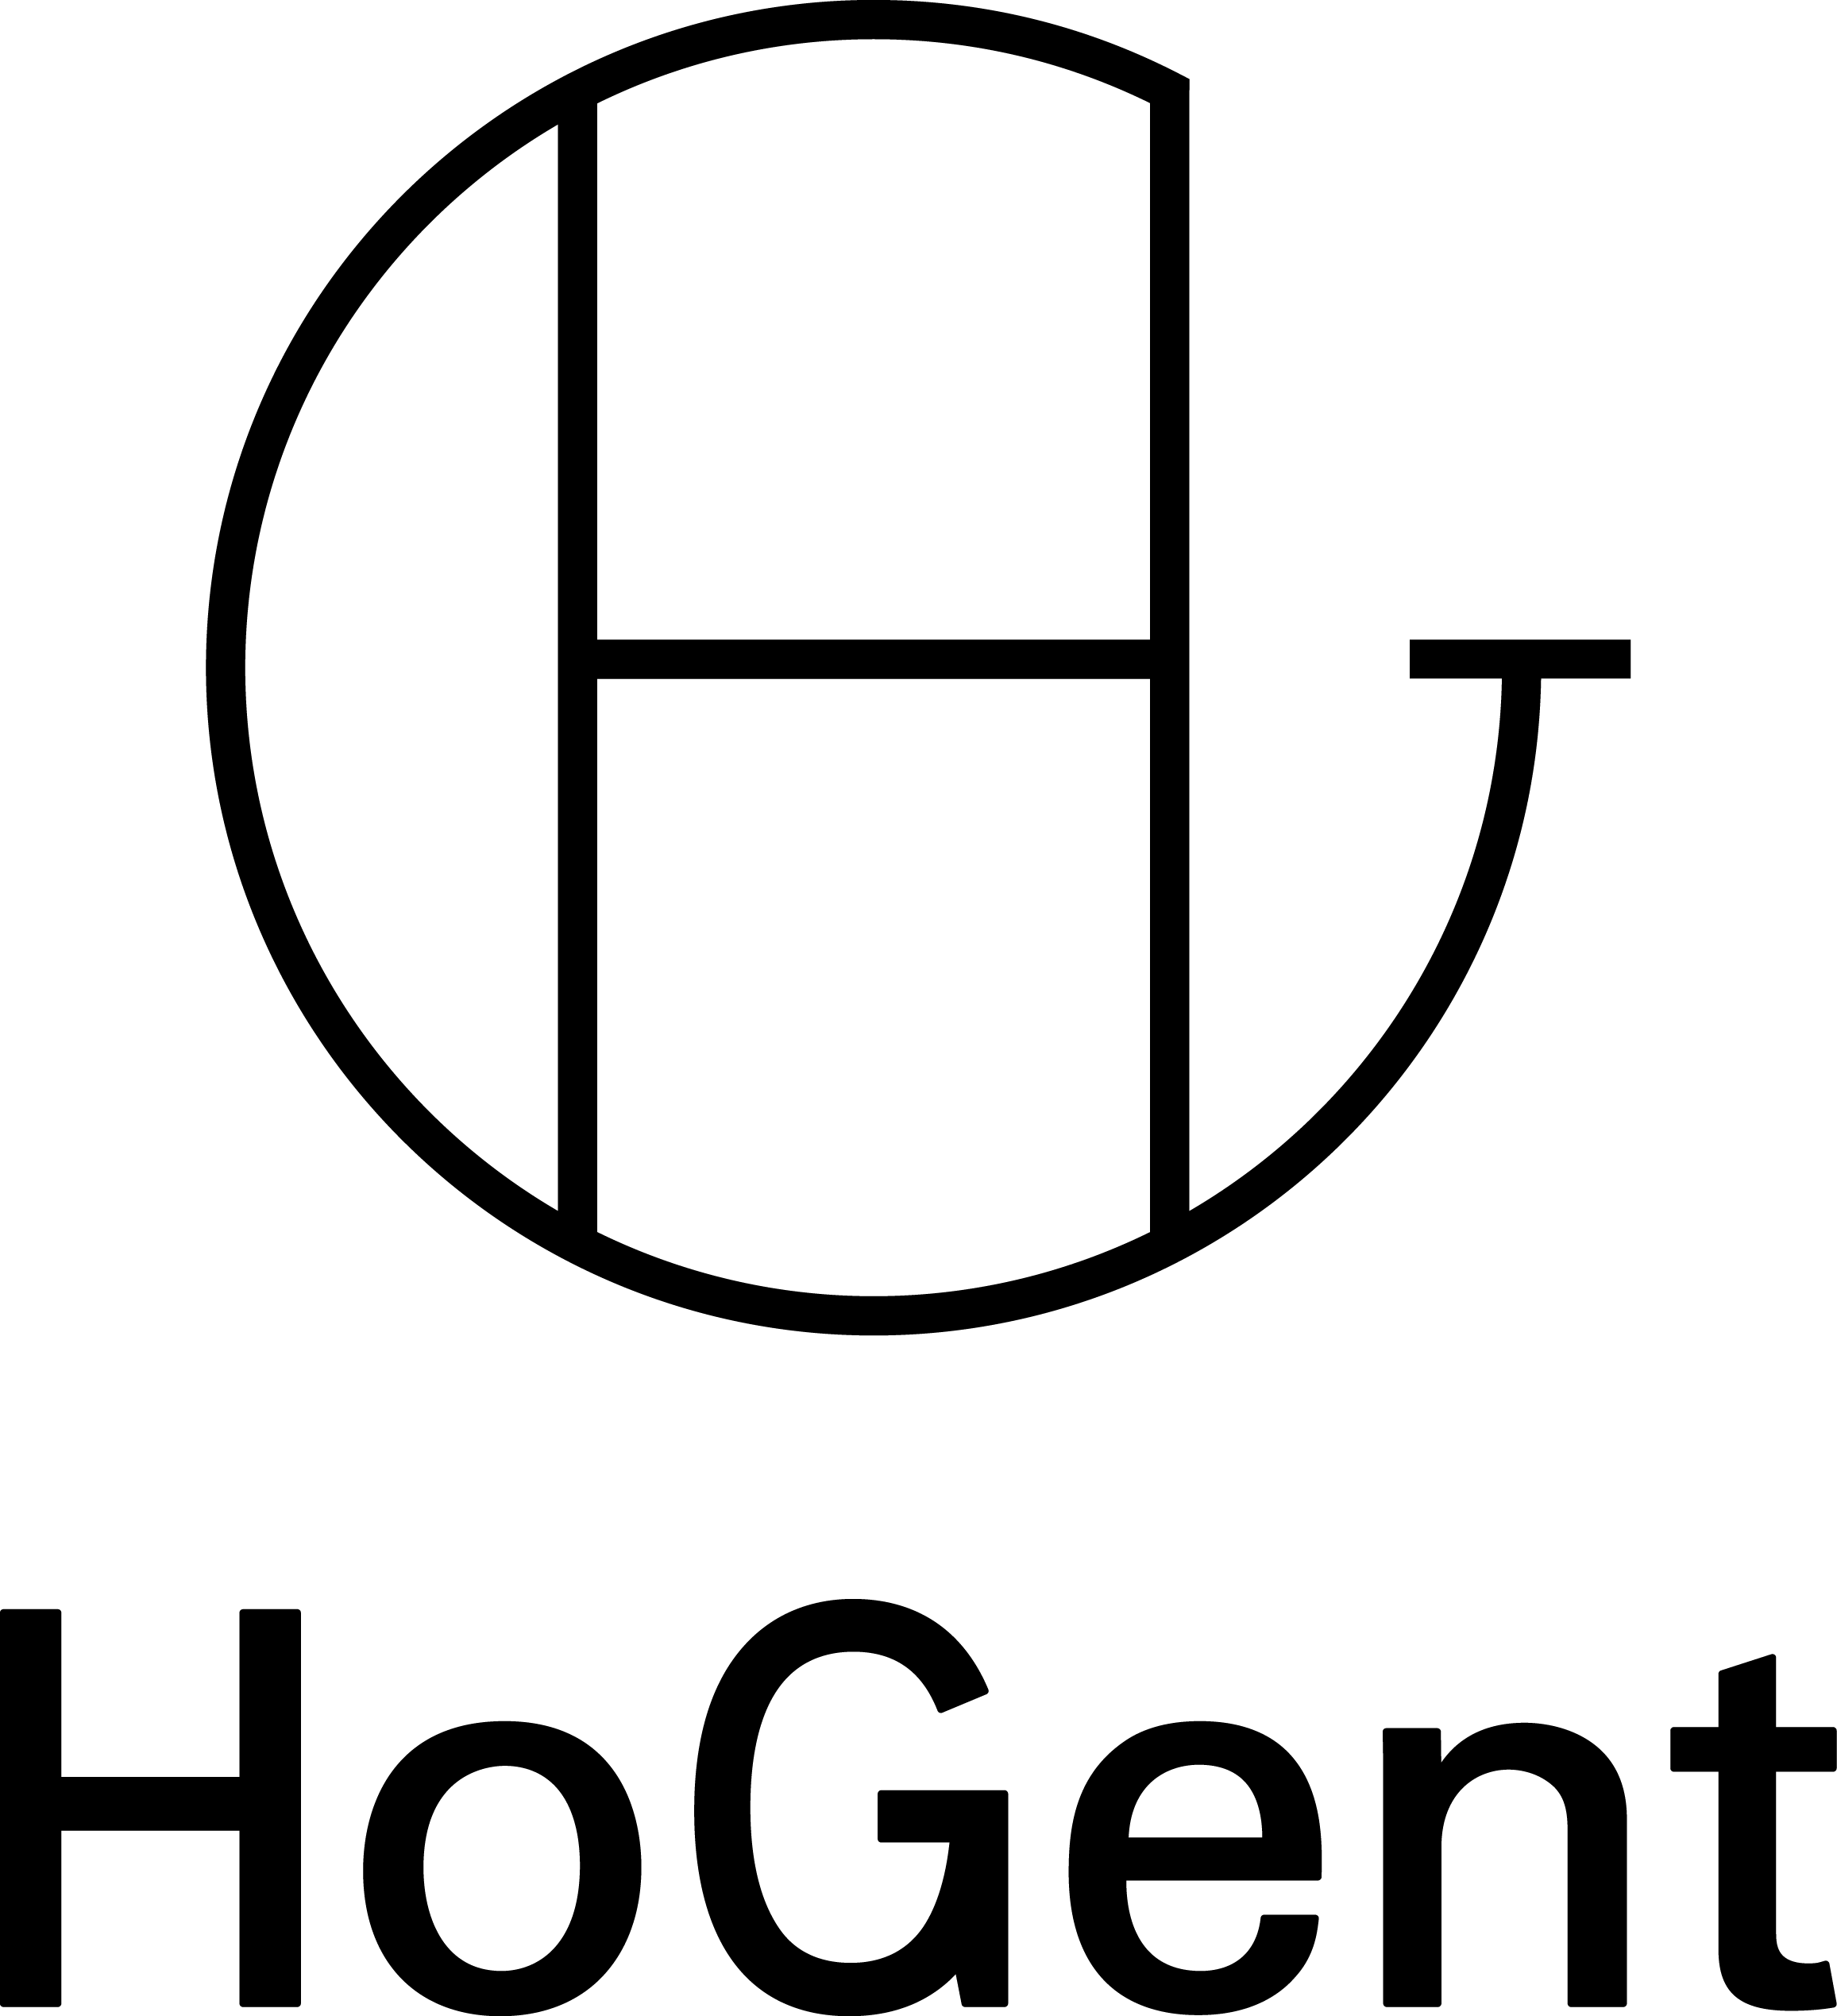
\includegraphics[width=2.5cm]{img/HG-beeldmerk-woordmerk}\\[.5cm]
    Faculteit Bedrijf en Organisatie\\[3cm]
    \titel
    \vfill
    \student\\[3.5cm]
    Scriptie voorgedragen tot het bekomen van de graad van\\professionele bachelor in de toegepaste informatica\\[2cm]
    Promotor:\\
    \promotor\\
    \ifdefempty{\copromotor}{\vspace{2.5cm}}{Co-promotor:\\\copromotor\\[2.5cm]}
    Instelling: \instelling\\[.5cm]
    Academiejaar: \academiejaar\\[.5cm]
    \ifcase \examenperiode \or Eerste \or Tweede \else Derde \fi examenperiode
    \endgroup

  \end{center}
  \restoregeometry
\end{titlepage}
  \emptypage
\begin{titlepage}
  \newgeometry{top=5.35cm,bottom=1.5cm,left=1.5cm,right=1.5cm}
  \begin{center}

    \begingroup
    \rmfamily
    \IfLanguageName{dutch}{Faculteit Bedrijf en Organisatie}{Faculty of Business and Information Management}\\[3cm]
    \titel
    \vfill
    \student\\[3.5cm]
    \IfLanguageName{dutch}{Scriptie voorgedragen tot het bekomen van de graad van\\professionele bachelor in de toegepaste informatica}{Thesis submitted in partial fulfillment of the requirements for the degree of\\professional bachelor of applied computer science}\\[2cm]
    Promotor:\\
    \promotor\\
    \ifdefempty{\copromotor}{\vspace{2.5cm}}{Co-promotor:\\\copromotor\\[2.5cm]}
    \IfLanguageName{dutch}{Instelling}{Institution}: \instelling\\[.5cm]
    \IfLanguageName{dutch}{Academiejaar}{Academic year}: \academiejaar\\[.5cm]
    \IfLanguageName{dutch}{%
    \ifcase \examenperiode \or Eerste \or Tweede \else Derde \fi examenperiode}{%
    \ifcase \examenperiode \or First \or Second \else Third \fi examination period}
    \endgroup

  \end{center}
  \restoregeometry
\end{titlepage}
}

%----------------------------------------------------------------------------------------
%	BIBLIOGRAPHY AND INDEX
%----------------------------------------------------------------------------------------

\usepackage[style=apa,backend=biber]{biblatex}
\usepackage{csquotes}
\DeclareLanguageMapping{dutch}{dutch-apa}
\addbibresource{bachproef-tin.bib} % BibTeX bibliography file
\defbibheading{bibempty}{}

\usepackage{calc} % For simpler calculation - used for spacing the index letter headings correctly
\usepackage{makeidx} % Required to make an index
\makeindex % Tells LaTeX to create the files required for indexing

%----------------------------------------------------------------------------------------
%	MAIN TABLE OF CONTENTS
%----------------------------------------------------------------------------------------

\usepackage{titletoc} % Required for manipulating the table of contents

\contentsmargin{0cm} % Removes the default margin

% Part text styling
\titlecontents{part}[0cm]
{\addvspace{20pt}\centering\large\bfseries}
{}
{}
{}

% Chapter text styling
\titlecontents{chapter}[1.25cm] % Indentation
{\addvspace{12pt}\large\sffamily\bfseries} % Spacing and font options for chapters
{\color{maincolor!60}\contentslabel[\Large\thecontentslabel]{1.25cm}\color{maincolor}} % Chapter number
{\color{maincolor}}
{\color{maincolor!60}\normalsize\;\titlerule*[.5pc]{.}\;\thecontentspage} % Page number

% Section text styling
\titlecontents{section}[1.25cm] % Indentation
{\addvspace{3pt}\sffamily\bfseries} % Spacing and font options for sections
{\contentslabel[\thecontentslabel]{1.25cm}} % Section number
{}
{\hfill\color{black}\thecontentspage} % Page number
[]

% Subsection text styling
\titlecontents{subsection}[1.25cm] % Indentation
{\addvspace{1pt}\sffamily\small} % Spacing and font options for subsections
{\contentslabel[\thecontentslabel]{1.25cm}} % Subsection number
{}
{\ \titlerule*[.5pc]{.}\;\thecontentspage} % Page number
[]

% List of figures
\titlecontents{figure}[0em]
{\addvspace{-5pt}\sffamily}
{\thecontentslabel\hspace*{1em}}
{}
{\ \titlerule*[.5pc]{.}\;\thecontentspage}
[]

% List of tables
\titlecontents{table}[0em]
{\addvspace{-5pt}\sffamily}
{\thecontentslabel\hspace*{1em}}
{}
{\ \titlerule*[.5pc]{.}\;\thecontentspage}
[]

%----------------------------------------------------------------------------------------
%	MINI TABLE OF CONTENTS IN PART HEADS
%----------------------------------------------------------------------------------------

% Chapter text styling
\titlecontents{lchapter}[0em] % Indenting
{\addvspace{15pt}\large\sffamily\bfseries} % Spacing and font options for chapters
{\color{maincolor}\contentslabel[\Large\thecontentslabel]{1.25cm}\color{maincolor}} % Chapter number
{}
{\color{maincolor}\normalsize\sffamily\bfseries\;\titlerule*[.5pc]{.}\;\thecontentspage} % Page number

% Section text styling
\titlecontents{lsection}[0em] % Indenting
{\sffamily\small} % Spacing and font options for sections
{\contentslabel[\thecontentslabel]{1.25cm}} % Section number
{}
{}

% Subsection text styling
\titlecontents{lsubsection}[.5em] % Indentation
{\normalfont\footnotesize\sffamily} % Font settings
{}
{}
{}

%----------------------------------------------------------------------------------------
%	PAGE HEADERS
%----------------------------------------------------------------------------------------

\usepackage{fancyhdr} % Required for header and footer configuration

\pagestyle{fancy}
\renewcommand{\chaptermark}[1]{\markboth{\sffamily\normalsize\bfseries\chaptername\ \thechapter.\ #1}{}} % Chapter text font settings
\renewcommand{\sectionmark}[1]{\markright{\sffamily\normalsize\thesection\hspace{5pt}#1}{}} % Section text font settings
\fancyhf{} \fancyhead[LE,RO]{\sffamily\normalsize\thepage} % Font setting for the page number in the header
\fancyhead[LO]{\rightmark} % Print the nearest section name on the left side of odd pages
\fancyhead[RE]{\leftmark} % Print the current chapter name on the right side of even pages
\renewcommand{\headrulewidth}{0.5pt} % Width of the rule under the header
\addtolength{\headheight}{2.5pt} % Increase the spacing around the header slightly
\renewcommand{\footrulewidth}{0pt} % Removes the rule in the footer
\fancypagestyle{plain}{\fancyhead{}\renewcommand{\headrulewidth}{0pt}} % Style for when a plain pagestyle is specified

% Removes the header from odd empty pages at the end of chapters
\makeatletter
\renewcommand{\cleardoublepage}{
\clearpage\ifodd\c@page\else
\hbox{}
\vspace*{\fill}
\thispagestyle{empty}
\newpage
\fi}

%----------------------------------------------------------------------------------------
%	THEOREM STYLES
%----------------------------------------------------------------------------------------

\usepackage{amsmath,amsfonts,amssymb,amsthm} % For math equations, theorems, symbols, etc

\newcommand{\intoo}[2]{\mathopen{]}#1\,;#2\mathclose{[}}
\newcommand{\ud}{\mathop{\mathrm{{}d}}\mathopen{}}
\newcommand{\intff}[2]{\mathopen{[}#1\,;#2\mathclose{]}}
\newtheorem{notation}{Notation}[chapter]

% Boxed/framed environments
\newtheoremstyle{maincolornumbox}% % Theorem style name
{0pt}% Space above
{0pt}% Space below
{\normalfont}% % Body font
{}% Indent amount
{\small\bf\sffamily\color{maincolor}}% % Theorem head font
{\;}% Punctuation after theorem head
{0.25em}% Space after theorem head
{\small\sffamily\color{maincolor}\thmname{#1}\nobreakspace\thmnumber{\@ifnotempty{#1}{}\@upn{#2}}% Theorem text (e.g. Theorem 2.1)
\thmnote{\nobreakspace\the\thm@notefont\sffamily\bfseries\color{black}---\nobreakspace#3.}} % Optional theorem note
\renewcommand{\qedsymbol}{$\blacksquare$}% Optional qed square

\newtheoremstyle{blacknumex}% Theorem style name
{5pt}% Space above
{5pt}% Space below
{\normalfont}% Body font
{} % Indent amount
{\small\bf\sffamily}% Theorem head font
{\;}% Punctuation after theorem head
{0.25em}% Space after theorem head
{\small\sffamily{\tiny\ensuremath{\blacksquare}}\nobreakspace\thmname{#1}\nobreakspace\thmnumber{\@ifnotempty{#1}{}\@upn{#2}}% Theorem text (e.g. Theorem 2.1)
\thmnote{\nobreakspace\the\thm@notefont\sffamily\bfseries---\nobreakspace#3.}}% Optional theorem note

\newtheoremstyle{blacknumbox} % Theorem style name
{0pt}% Space above
{0pt}% Space below
{\normalfont}% Body font
{}% Indent amount
{\small\bf\sffamily}% Theorem head font
{\;}% Punctuation after theorem head
{0.25em}% Space after theorem head
{\small\sffamily\thmname{#1}\nobreakspace\thmnumber{\@ifnotempty{#1}{}\@upn{#2}}% Theorem text (e.g. Theorem 2.1)
\thmnote{\nobreakspace\the\thm@notefont\sffamily\bfseries---\nobreakspace#3.}}% Optional theorem note

% Non-boxed/non-framed environments
\newtheoremstyle{maincolornum}% % Theorem style name
{5pt}% Space above
{5pt}% Space below
{\normalfont}% % Body font
{}% Indent amount
{\small\bf\sffamily\color{maincolor}}% % Theorem head font
{\;}% Punctuation after theorem head
{0.25em}% Space after theorem head
{\small\sffamily\color{maincolor}\thmname{#1}\nobreakspace\thmnumber{\@ifnotempty{#1}{}\@upn{#2}}% Theorem text (e.g. Theorem 2.1)
\thmnote{\nobreakspace\the\thm@notefont\sffamily\bfseries\color{black}---\nobreakspace#3.}} % Optional theorem note
\renewcommand{\qedsymbol}{$\blacksquare$}% Optional qed square
\makeatother

% Defines the theorem text style for each type of theorem to one of the three styles above
\newcounter{dummy}
\numberwithin{dummy}{section}
\theoremstyle{maincolornumbox}
\newtheorem{theoremeT}[dummy]{Theorem}
\newtheorem{problem}{Problem}[chapter]
\newtheorem{exerciseT}{Exercise}[chapter]
\theoremstyle{blacknumex}
\newtheorem{exampleT}{Example}[chapter]
\theoremstyle{blacknumbox}
\newtheorem{vocabulary}{Vocabulary}[chapter]
\newtheorem{definitionT}{Definition}[section]
\newtheorem{corollaryT}[dummy]{Corollary}
\theoremstyle{maincolornum}
\newtheorem{proposition}[dummy]{Proposition}

%----------------------------------------------------------------------------------------
%	DEFINITION OF COLORED BOXES
%----------------------------------------------------------------------------------------

\RequirePackage[framemethod=default]{mdframed} % Required for creating the theorem, definition, exercise and corollary boxes

% Theorem box
\newmdenv[skipabove=7pt,
skipbelow=7pt,
backgroundcolor=black!5,
linecolor=maincolor,
innerleftmargin=5pt,
innerrightmargin=5pt,
innertopmargin=5pt,
leftmargin=0cm,
rightmargin=0cm,
innerbottommargin=5pt]{tBox}

% Exercise box
\newmdenv[skipabove=7pt,
skipbelow=7pt,
rightline=false,
leftline=true,
topline=false,
bottomline=false,
backgroundcolor=maincolor!10,
linecolor=maincolor,
innerleftmargin=5pt,
innerrightmargin=5pt,
innertopmargin=5pt,
innerbottommargin=5pt,
leftmargin=0cm,
rightmargin=0cm,
linewidth=4pt]{eBox}

% Definition box
\newmdenv[skipabove=7pt,
skipbelow=7pt,
rightline=false,
leftline=true,
topline=false,
bottomline=false,
linecolor=maincolor,
innerleftmargin=5pt,
innerrightmargin=5pt,
innertopmargin=0pt,
leftmargin=0cm,
rightmargin=0cm,
linewidth=4pt,
innerbottommargin=0pt]{dBox}

% Corollary box
\newmdenv[skipabove=7pt,
skipbelow=7pt,
rightline=false,
leftline=true,
topline=false,
bottomline=false,
linecolor=gray,
backgroundcolor=black!5,
innerleftmargin=5pt,
innerrightmargin=5pt,
innertopmargin=5pt,
leftmargin=0cm,
rightmargin=0cm,
linewidth=4pt,
innerbottommargin=5pt]{cBox}

% Creates an environment for each type of theorem and assigns it a theorem text style from the "Theorem Styles" section above and a colored box from above
\newenvironment{theorem}{\begin{tBox}\begin{theoremeT}}{\end{theoremeT}\end{tBox}}
\newenvironment{exercise}{\begin{eBox}\begin{exerciseT}}{\hfill{\color{maincolor}\tiny\ensuremath{\blacksquare}}\end{exerciseT}\end{eBox}}
\newenvironment{definition}{\begin{dBox}\begin{definitionT}}{\end{definitionT}\end{dBox}}
\newenvironment{example}{\begin{exampleT}}{\hfill{\tiny\ensuremath{\blacksquare}}\end{exampleT}}
\newenvironment{corollary}{\begin{cBox}\begin{corollaryT}}{\end{corollaryT}\end{cBox}}

%----------------------------------------------------------------------------------------
%	REMARK ENVIRONMENT
%----------------------------------------------------------------------------------------

\newenvironment{remark}{\par\vspace{10pt}\small % Vertical white space above the remark and smaller font size
\begin{list}{}{
\leftmargin=35pt % Indentation on the left
\rightmargin=25pt}\item\ignorespaces % Indentation on the right
\makebox[-2.5pt]{\begin{tikzpicture}[overlay]
\node[draw=maincolor!60,line width=1pt,circle,fill=maincolor!25,font=\sffamily\bfseries,inner sep=2pt,outer sep=0pt] at (-15pt,0pt){\textcolor{maincolor}{R}};\end{tikzpicture}} % Orange R in a circle
\advance\baselineskip -1pt}{\end{list}\vskip5pt} % Tighter line spacing and white space after remark

%----------------------------------------------------------------------------------------
%	SECTION NUMBERING IN THE MARGIN
%----------------------------------------------------------------------------------------

\makeatletter
\renewcommand{\@seccntformat}[1]{\llap{\textcolor{maincolor}{\csname the#1\endcsname}\hspace{1em}}}
\renewcommand{\section}{\@startsection{section}{1}{\z@}
{-4ex \@plus -1ex \@minus -.4ex}
{1ex \@plus.2ex }
{\normalfont\large\sffamily\bfseries}}
\renewcommand{\subsection}{\@startsection {subsection}{2}{\z@}
{-3ex \@plus -0.1ex \@minus -.4ex}
{0.5ex \@plus.2ex }
{\normalfont\sffamily\bfseries}}
\renewcommand{\subsubsection}{\@startsection {subsubsection}{3}{\z@}
{-2ex \@plus -0.1ex \@minus -.2ex}
{.2ex \@plus.2ex }
{\normalfont\small\sffamily\bfseries}}
\renewcommand\paragraph{\@startsection{paragraph}{4}{\z@}
{-2ex \@plus-.2ex \@minus .2ex}
{.1ex}
{\normalfont\small\sffamily\bfseries}}

%----------------------------------------------------------------------------------------
%	PART HEADINGS
%----------------------------------------------------------------------------------------

% numbered part in the table of contents
\newcommand{\@mypartnumtocformat}[2]{%
\setlength\fboxsep{0pt}%
\noindent\colorbox{maincolor!20}{\strut\parbox[c][.7cm]{\ecart}{\color{maincolor!70}\Large\sffamily\bfseries\centering#1}}\hskip\esp\colorbox{maincolor!40}{\strut\parbox[c][.7cm]{\linewidth-\ecart-\esp}{\Large\sffamily\centering#2}}}%
%%%%%%%%%%%%%%%%%%%%%%%%%%%%%%%%%%
% unnumbered part in the table of contents
\newcommand{\@myparttocformat}[1]{%
\setlength\fboxsep{0pt}%
\noindent\colorbox{maincolor!40}{\strut\parbox[c][.7cm]{\linewidth}{\Large\sffamily\centering#1}}}%
%%%%%%%%%%%%%%%%%%%%%%%%%%%%%%%%%%
\newlength\esp
\setlength\esp{4pt}
\newlength\ecart
\setlength\ecart{1.2cm-\esp}
\newcommand{\thepartimage}{}%
\newcommand{\partimage}[1]{\renewcommand{\thepartimage}{#1}}%
\def\@part[#1]#2{%
\ifnum \c@secnumdepth >-4\relax%
\refstepcounter{part}%
\addcontentsline{toc}{part}{\texorpdfstring{\protect\@mypartnumtocformat{\thepart}{#1}}{\partname~\thepart\ ---\ #1}}
\else%
\addcontentsline{toc}{part}{\texorpdfstring{\protect\@myparttocformat{#1}}{#1}}%
\fi%
\startcontents%
\markboth{}{}%
{\thispagestyle{empty}%
\begin{tikzpicture}[remember picture,overlay]%
\node at (current page.north west){\begin{tikzpicture}[remember picture,overlay]%
\fill[maincolor!20](0cm,0cm) rectangle (\paperwidth,-\paperheight);
\node[anchor=north] at (4cm,-3.25cm){\color{maincolor!40}\fontsize{220}{100}\sffamily\bfseries\@Roman\c@part};
\node[anchor=south east] at (\paperwidth-1cm,-\paperheight+1cm){\parbox[t][][t]{8.5cm}{
\printcontents{l}{0}{\setcounter{tocdepth}{3}}%
}};
\node[anchor=north east] at (\paperwidth-1.5cm,-3.25cm){\parbox[t][][t]{15cm}{\strut\raggedleft\color{white}\fontsize{30}{30}\sffamily\bfseries#2}};
\end{tikzpicture}};
\end{tikzpicture}}%
\@endpart}
\def\@spart#1{%
\startcontents%
\phantomsection
{\thispagestyle{empty}%
\begin{tikzpicture}[remember picture,overlay]%
\node at (current page.north west){\begin{tikzpicture}[remember picture,overlay]%
\fill[maincolor!20](0cm,0cm) rectangle (\paperwidth,-\paperheight);
\node[anchor=north east] at (\paperwidth-1.5cm,-3.25cm){\parbox[t][][t]{15cm}{\strut\raggedleft\color{white}\fontsize{30}{30}\sffamily\bfseries#1}};
\end{tikzpicture}};
\end{tikzpicture}}
\addcontentsline{toc}{part}{\texorpdfstring{%
\setlength\fboxsep{0pt}%
\noindent\protect\colorbox{maincolor!40}{\strut\protect\parbox[c][.7cm]{\linewidth}{\Large\sffamily\protect\centering #1\quad\mbox{}}}}{#1}}%
\@endpart}
\def\@endpart{\vfil\newpage
\if@twoside
\if@openright
\null
\thispagestyle{empty}%
\newpage
\fi
\fi
\if@tempswa
\twocolumn
\fi}

%----------------------------------------------------------------------------------------
%	CHAPTER HEADINGS
%----------------------------------------------------------------------------------------

% A switch to conditionally include a picture, implemented by  Christian Hupfer
\newif\ifusechapterimage
\usechapterimagetrue
\newcommand{\thechapterimage}{}%
\newcommand{\chapterimage}[1]{\ifusechapterimage\renewcommand{\thechapterimage}{#1}\fi}%
\def\@makechapterhead#1{%
{\parindent \z@ \raggedright \normalfont
\ifnum \c@secnumdepth >\m@ne
\if@mainmatter
\begin{tikzpicture}[remember picture,overlay]
\node at (current page.north west)
{\begin{tikzpicture}[remember picture,overlay]
\node[anchor=north west,inner sep=0pt] at (0,0) {\ifusechapterimage\includegraphics[width=\paperwidth]{\thechapterimage}\fi};
\draw[anchor=west] (\Gm@lmargin,-9cm) node [line width=2pt,rounded corners=15pt,draw=maincolor,fill=white,fill opacity=0.5,inner sep=15pt]{\strut\makebox[22cm]{}};
\draw[anchor=west] (\Gm@lmargin+.3cm,-9cm) node {\huge\sffamily\bfseries\color{black}\thechapter. #1\strut};
\end{tikzpicture}};
\end{tikzpicture}
\else
\begin{tikzpicture}[remember picture,overlay]
\node at (current page.north west)
{\begin{tikzpicture}[remember picture,overlay]
\node[anchor=north west,inner sep=0pt] at (0,0) {\ifusechapterimage\includegraphics[width=\paperwidth]{\thechapterimage}\fi};
\draw[anchor=west] (\Gm@lmargin,-9cm) node [line width=2pt,rounded corners=15pt,draw=maincolor,fill=white,fill opacity=0.5,inner sep=15pt]{\strut\makebox[22cm]{}};
\draw[anchor=west] (\Gm@lmargin+.3cm,-9cm) node {\huge\sffamily\bfseries\color{black}#1\strut};
\end{tikzpicture}};
\end{tikzpicture}
\fi\fi\par\vspace*{270\p@}}}

%-------------------------------------------

\def\@makeschapterhead#1{%
\begin{tikzpicture}[remember picture,overlay]
\node at (current page.north west)
{\begin{tikzpicture}[remember picture,overlay]
\node[anchor=north west,inner sep=0pt] at (0,0) {\ifusechapterimage\includegraphics[width=\paperwidth]{\thechapterimage}\fi};
\draw[anchor=west] (\Gm@lmargin,-9cm) node [line width=2pt,rounded corners=15pt,draw=maincolor,fill=white,fill opacity=0.5,inner sep=15pt]{\strut\makebox[22cm]{}};
\draw[anchor=west] (\Gm@lmargin+.3cm,-9cm) node {\huge\sffamily\bfseries\color{black}#1\strut};
\end{tikzpicture}};
\end{tikzpicture}
\par\vspace*{270\p@}}
\makeatother

%----------------------------------------------------------------------------------------
%	HYPERLINKS IN THE DOCUMENTS
%----------------------------------------------------------------------------------------

\usepackage{hyperref}
\hypersetup{hidelinks,backref=true,pagebackref=true,hyperindex=true,colorlinks=false,breaklinks=true,urlcolor= maincolor,bookmarks=true,bookmarksopen=false,pdftitle={Title},pdfauthor={Author}}
\usepackage{bookmark}
\bookmarksetup{
open,
numbered,
addtohook={%
\ifnum\bookmarkget{level}=0 % chapter
\bookmarksetup{bold}%
\fi
\ifnum\bookmarkget{level}=-1 % part
\bookmarksetup{color=maincolor,bold}%
\fi
}
}

%----------------------------------------------------------------------------------------
%	Java source code
%----------------------------------------------------------------------------------------

% Commando voor invoegen Java-broncodebestanden (dank aan Niels Corneille)
% Gebruik:
%   \codefragment{source/MijnKlasse.java}{Uitleg bij de code}
%
% Je kan dit aanpassen aan de taal die je zelf het meeste gebruikt in je
% bachelorproef.
\newcommand{\codefragment}[2]{ \lstset{%
  language=java,
  breaklines=true,
  float=th,
  caption={#2},
  basicstyle=\scriptsize,
  frame=single,
  extendedchars=\true
}
\lstinputlisting{#1}}

% Leeg blad
\newcommand{\emptypage}{%
\newpage
\thispagestyle{empty}
\mbox{}
\newpage
}


%%---------- Documenteigenschappen --------------------------------------------
%% TODO: Vul dit aan met je eigen info:

% Je eigen naam
\newcommand{\student}{Thomas Ledoux}

% De naam van je promotor (lector van de opleiding)
\newcommand{\promotor}{Jens Buysse}

% De naam van je co-promotor. Als je promotor ook je opdrachtgever is en je
% dus ook inhoudelijk begeleidt (en enkel dan!), mag je dit leeg laten.
\newcommand{\copromotor}{}

% Indien je bachelorproef in opdracht van/in samenwerking met een bedrijf of
% externe organisatie geschreven is, geef je hier de naam. Zoniet laat je dit
% zoals het is.
\newcommand{\instelling}{---}

% De titel van het rapport/bachelorproef
\newcommand{\titel}{Hoe beperken ontwikkelaars de schijfruimte ingenomen door mobiele applicaties voor Android Wear?}

% Datum van indienen (gebruik telkens de deadline, ook al geef je eerder af)
\newcommand{\datum}{27 mei 2017}

% Academiejaar
\newcommand{\academiejaar}{2016-2017}

% Examenperiode
%  - 1e semester = 1e examenperiode => 1
%  - 2e semester = 2e examenperiode => 2
%  - tweede zit  = 3e examenperiode => 3
\newcommand{\examenperiode}{2}

%%=============================================================================
%% Inhoud document
%%=============================================================================

\begin{document}

%---------- Taalselectie ------------------------------------------------------
%% Als je je bachelorproef in het Engels schrijft, haal dan onderstaande regel
%% uit commentaar. Let op: de tekst op de voorkaft blijft in het Nederlands, en
%% dat is ook de bedoeling!
%\selectlanguage{english}

%---------- Titelblad ---------------------------------------------------------
\inserttitlepage

%---------- Samenvatting, voorwoord -------------------------------------------
\usechapterimagefalse
%%=============================================================================
%% Samenvatting
%%=============================================================================

%% TODO: De "abstract" of samenvatting is een kernachtige (~ 1 blz. voor een
%% thesis) synthese van het document.
%%
%% Deze aspecten moeten zeker aan bod komen:
%% - Context: waarom is dit werk belangrijk?
%% - Nood: waarom moest dit onderzocht worden?
%% - Taak: wat heb je precies gedaan?
%% - Object: wat staat in dit document geschreven?
%% - Resultaat: wat was het resultaat?
%% - Conclusie: wat is/zijn de belangrijkste conclusie(s)?
%% - Perspectief: blijven er nog vragen open die in de toekomst nog kunnen
%%    onderzocht worden? Wat is een mogelijk vervolg voor jouw onderzoek?
%%
%% LET OP! Een samenvatting is GEEN voorwoord!

%%---------- Nederlandse samenvatting -----------------------------------------
%%
%% TODO: Als je je bachelorproef in het Engels schrijft, moet je eerst een
%% Nederlandse samenvatting invoegen. Haal daarvoor onderstaande code uit
%% commentaar.
%% Wie zijn bachelorproef in het Nederlands schrijft, kan dit negeren en heel
%% deze sectie verwijderen.

\IfLanguageName{english}{%
\selectlanguage{dutch}
\chapter*{Samenvatting}
\lipsum[1-4]
\selectlanguage{english}
}{}

%%---------- Samenvatting -----------------------------------------------------
%%
%% De samenvatting in de hoofdtaal van het document

\chapter*{\IfLanguageName{dutch}{Samenvatting}{Abstract}}


%%=============================================================================
%% Voorwoord
%%=============================================================================

\chapter*{Voorwoord}
\label{ch:voorwoord}

%% TODO:
%% Het voorwoord is het enige deel van de bachelorproef waar je vanuit je
%% eigen standpunt (``ik-vorm'') mag schrijven. Je kan hier bv. motiveren
%% waarom jij het onderwerp wil bespreken.
%% Vergeet ook niet te bedanken wie je geholpen/gesteund/... heeft

Ik zou graag deze gelegenheid nemen om enkele mensen te bedanken. 
Als eerste wil ik mijn promotor, Dr. Jens Buysse bedanken voor de
kans die hij me bood om deze bachelorproef onder zijn promotorschap te volbrengen, voor
de feedback \& de aangename begeleiding tijdens het semester. En ook mijn co-promotor Joris Missiaen verdient zeker een dankjewel voor de inhoudelijke ondersteuning, waardoor mijn bachelorproef er zeker anders had uitgezien.
Natuurlijk was ik nooit zo ver gekomen zonder de onvoorwaardelijke steun van
mijn twee lieve ouders. Zowel financieel als emotioneel zijn zij er 3 jaar lang volledig
voor mij geweest. Voor het nalezen van teksten, het warme weekendnest en het oneindige vertrouwen dat ze in mij stelden
gedurende mijn volledige opleiding, dankjewel! Ook mijn vriendin Louise wil ik bedanken voor het geduld, de gerustellingen en de ondersteuning op elke manier. Louise geloofde er altijd in dat ik deze bachelorproef tot een goed einde zou brengen, en wist mij in dit geloof meer te trekken.

%---------- Inhoudstafel ------------------------------------------------------
\pagestyle{empty} % No headers
\tableofcontents % Print the table of contents itself
\cleardoublepage % Forces the first chapter to start on an odd page so it's on the right
\pagestyle{fancy} % Print headers again

%---------- Lijst afkortingen, termen -----------------------------------------
%% Als je een lijst van afkortingen of termen wil toevoegen, dan hoort die
%% hier thuis. Gebruik bijvoorbeeld de ``glossaries'' package.

%%---------- Kern -------------------------------------------------------------

%%=============================================================================
%% Inleiding
%%=============================================================================

\chapter{Inleiding}
\label{ch:inleiding}


\section{Stand van zaken}
\label{sec:stand-van-zaken}

%% TODO: deze sectie (die je kan opsplitsen in verschillende secties) bevat je
%% literatuurstudie. Vergeet niet telkens je bronnen te vermelden!

Er zijn momenteel al veel technieken ontwikkeld en opgelijst door \textcite{google} om de grootte van applicaties voor Android te beperken. Er bestaat echter geen studie die het effect van deze technieken aantoont op de grootte van de applicaties en de performantie van de applicaties. Er bestaan ook bepaalde tools om de code van de applicatie te optimaliseren, zoals Proguard. ProGuard is de populairste optimalizator voor Java bytecode. De tool kan Java en Android applicaties tot 90 procent kleiner maken en tot 20 procent sneller. ProGuard voorziet ook minimale bescherming tegen reverse engineering door het  verdoezelen van de namen van klassen, velden en methodes.

\section{Probleemstelling en Onderzoeksvragen}
\label{sec:onderzoeksvragen}

%% TODO:
%% Uit je probleemstelling moet duidelijk zijn dat je onderzoek een meerwaarde
%% heeft voor een concrete doelgroep (bv. een bedrijf).
%%
%% Wees zo concreet mogelijk bij het formuleren van je
%% onderzoeksvra(a)g(en). Een onderzoeksvraag is trouwens iets waar nog
%% niemand op dit moment een antwoord heeft (voor zover je kan nagaan).
De voorbije jaren hebben wearable devices meer en meer aan belang gewonnen in het dagelijks leven. Volgens onderzoek van IDC\cite{apew} werd het aantal verkochte wearable devices wereldwijd geschat op 20.1 miljoen, waarvan 22.9 procent Android Wear als operating system gebruikt. IDC voorspelt tegen 2020 dat er 54.6 miljoen wearable devices verkocht zullen worden, waarvan 41.8 procent Android Wear als operating system zal gebruiken. Elk noemenswaardig bedrijf heeft tegenwoordig een app laten ontwikkelen die ook op wearable devices kan gebruikt worden om zoveel mogelijk van deze mobiele gebruikers te bereiken. Hiermee gaat echter gepaard dat gebruikers meer en meer apps willen installeren op hun wearables, terwijl deze slechts over een beperkte schijfruimte beschikken. Daarom moeten de ontwikkelaars van deze mobiele applicaties ervoor zorgen dat de grootte van hun applicaties zoveel mogelijk beperkt wordt, zodat mobiele toestellen niet zonder vrije schijfruimte komen te staan. Een bijkomend probleem voor de bedrijven is dat gebruikers een beperktere set van apps zullen installeren, en er dus een grotere kans is dat sommige apps niet meer geïnstalleerd worden en er dus minder omzet wordt behaald. De bedrijven die mobiele apps laten ontwikkelen, zullen hier rekening mee moeten houden en bijvoorbeeld meer diensten in de cloud moeten aanbieden, om zo de lokaal gebruikte schijfruimte te beperken. Om dit na te gaan, zal onderzoek gedaan worden naar de applicaties van enkele van de populairste en meestgebruikte apps, zoals Spotify, Tinder en WhatsApp. In het onderzoek zal de focus gelegd worden op de gebruikte technieken bij ontwikkeling voor Android Wear


\section{Opzet van deze bachelorproef}
\label{sec:opzet-bachelorproef}

%% TODO: Het is gebruikelijk aan het einde van de inleiding een overzicht te
%% geven van de opbouw van de rest van de tekst. Deze sectie bevat al een aanzet
%% die je kan aanvullen/aanpassen in functie van je eigen tekst.

%%De rest van deze bachelorproef is als volgt opgebouwd:

%%In Hoofdstuk~\ref{ch:methodologie} wordt de methodologie toegelicht en worden de gebruikte onderzoekstechnieken besproken om een antwoord te kunnen formuleren op de onderzoeksvragen.

%% TODO: Vul hier aan voor je eigen hoofstukken, één of twee zinnen per hoofdstuk

%%In Hoofdstuk~\ref{ch:conclusie}, tenslotte, wordt de conclusie gegeven en een antwoord geformuleerd op de onderzoeksvragen. Daarbij wordt ook een aanzet gegeven voor toekomstig onderzoek binnen dit domein.




%%=============================================================================
%% Methodologie
%%=============================================================================

\chapter{Methodologie}
\label{ch:methodologie}

%% TODO: Hoe ben je te werk gegaan? Verdeel je onderzoek in grote fasen, en
%% licht in elke fase toe welke stappen je gevolgd hebt. Verantwoord waarom je
%% op deze manier te werk gegaan bent. Je moet kunnen aantonen dat je de best
%% mogelijke manier toegepast hebt om een antwoord te vinden op de
%% onderzoeksvraag.

\section{Literatuurstudie Android Wear}
\label{sec:androidwear}
Android Wear is Google's platform voor wearables. Een wearable wordt beschreven als een computer of geavanceerd elektronisch toestel dat geïncorporeerd is in een accessoire gedragen op het lichaam of in een kledingstuk \autocite{Dictionary}.
We lijsten enkele van de  belangrijkste kenmerken van Android Wear op \autocite{Techradar}.
Android Wear is gebouwd voor kleinere toestellen en met hands-free gebruik in het achterhoofd. Het maakt de toegang tot enkele van uw smartphone's makkelijkste functionaliteiten zo makkelijk als kijken naar uw pols. Het is vooral bedoeld om de notificaties van uw smartphone makkelijk te weergeven zodat niet elke keer gezocht moet worden naar de smartphone in de broekzak. Gebaseerd op uw Google zoekopdrachten zullen real-time scores van uw favoriete sportteam, verkeerscondities of afspraken in uw agenda weergeven worden. Als het Android Wear toestel NFC (Near Field Communication) ingebouwd heeft, kan er in verschillende landen (momenteel Australië, Hong Kong, Ierland, Japan, Nieuw-Zeeland, Polen, Singapore, Verenigd Koninkrijk en de Verenigde Staten) ook met de wearable betaald worden via Android Pay \autocite{Androidpay} Ook spraakherkenning kon niet ontbreken in de Android Software. Door deze technologie kan je de op de wearable spraakherkenning activeren door "Okay, Google" te zeggen of door de aanknop ingedrukt te houden. Google Assistant zal u hierop verderhelpen. Android Wear is compatibel met smartphones die werken op Android 4.3 en hoger of iOS 9 en hoger. Eén van de belangrijkste app-categorieën op Android Wear zijn de gezondheidsapps. Hiervoor wordt standaard gebruik gemaakt van Google Fit. Met Google Fit kan je kiezen tussen verschillende workouts tijdens het sporten, of bijvoorbeeld een dagelijks doel instellen voor het aantal stappen dat u wil nemen.  
\begin{figure}[H]
	\centering
	\caption{\textit{Enkele voorbeelden van smartwatches gebruikmakend van Android Wear}}
	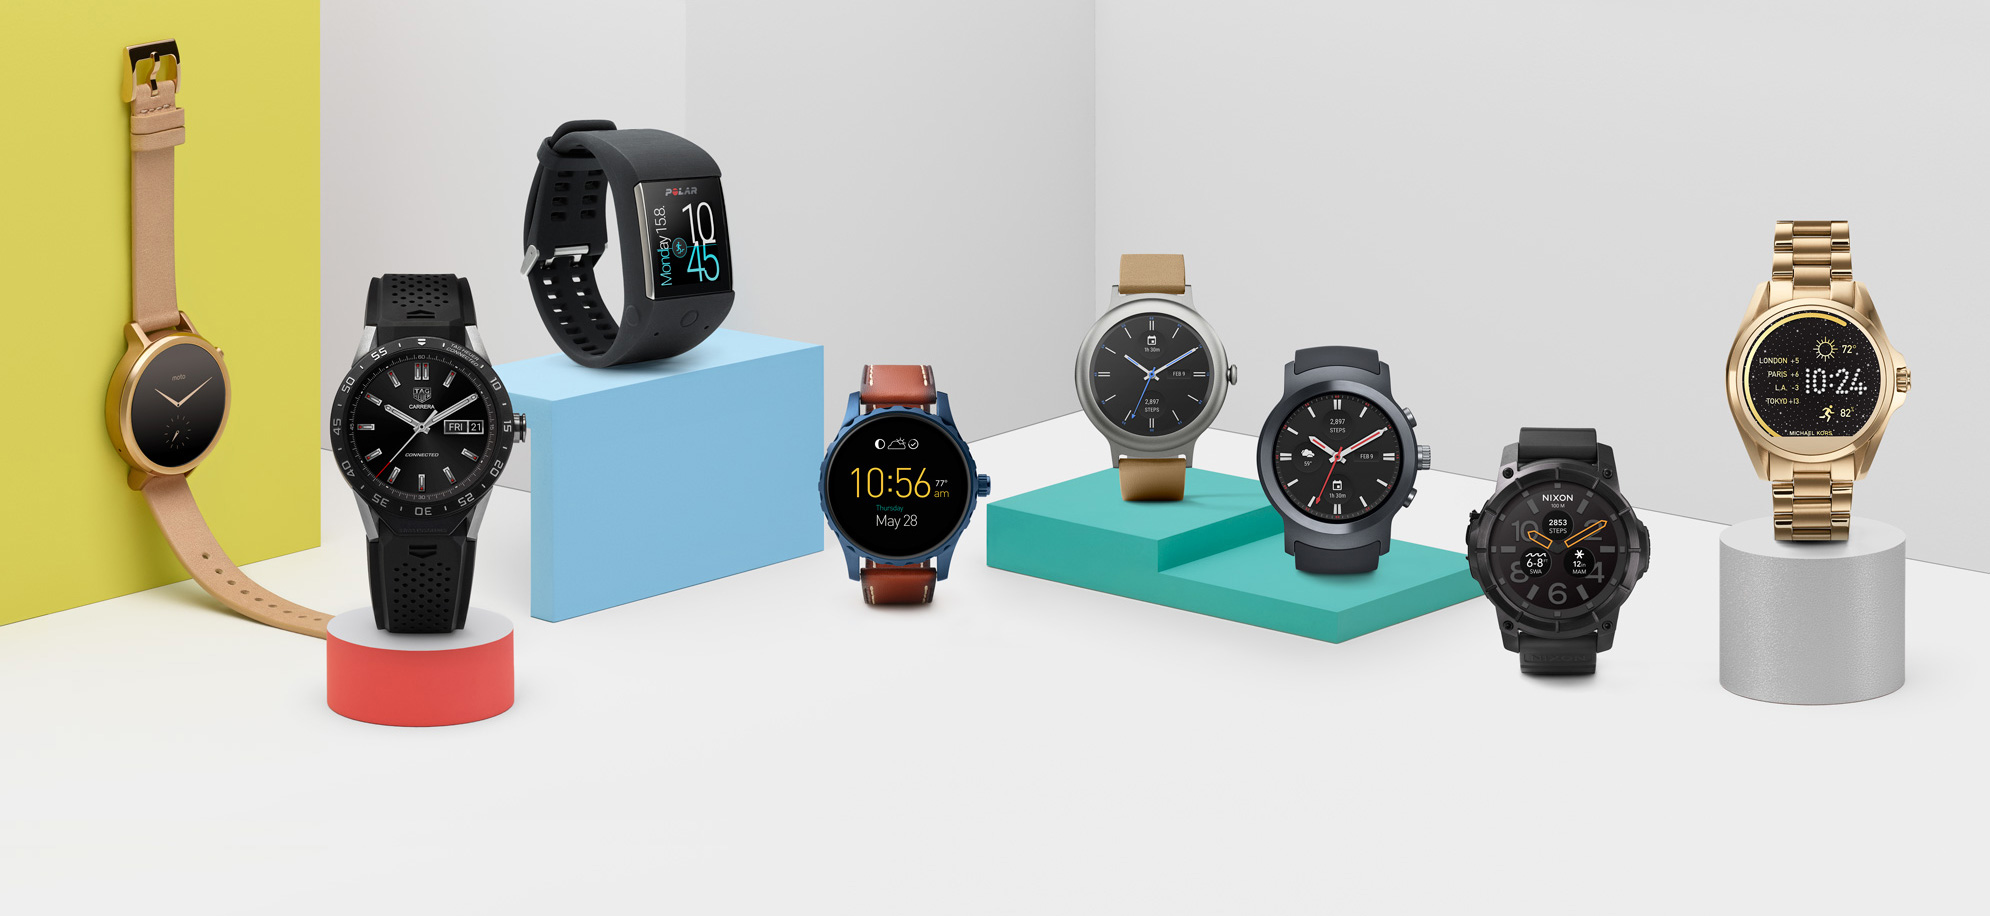
\includegraphics[width=10cm, height=10cm, keepaspectratio]{img/WearExamples}\\[.5cm]
\end{figure}
%% TODO:
%% Uit je probleemstelling moet duidelijk zijn dat je onderzoek een meerwaarde
%% heeft voor een concrete doelgroep (bv. een bedrijf).
%%
%% Wees zo concreet mogelijk bij het formuleren van je
%% onderzoeksvra(a)g(en). Een onderzoeksvraag is trouwens iets waar nog
%% niemand op dit moment een antwoord heeft (voor zover je kan nagaan).
\subsection{Wat is een APK en uit wat bestaat dit?}
APK staat voor Android Application Package. Een APK is een applicatiebestand klaar voor installatie op een Android-toestel. Het gecompresseerde APK bestand, een ZIP archief in JAR-formaat, wordt gedistribueerd naar Android gebruikers voor de installatie op hun smartphone, tablet of wearable \autocite{PCMag}.
Een APK bestand bestaat normaliter uit volgende elementen : 
\subsubsection{Elementen APK}
\begin{enumerate}
	\setlength\itemsep{2em}
	\item \textbf{classes.dex} \newline
	Bevat gecompileerde applicatiecode, getransformeerd naar een DEX bytecode. Het is mogelijk dat er meerdere DEX bestanden in de APK staan als er multidex gebruikt wordt om de 65536 limiet te overkomen. Vanaf Android 5.0, met de introductie van ART runtime, worden deze bestanden gecompileerd naar OAT bestanden door de compiler bij de installatie en worden deze op de data partitie van het toestel geplaatst. 
	\item \textbf{res/} \newline
	Deze folder bevat de meeste XML-bestanden en drawables (bijvoorbeeld PNG- of JPEG-bestanden) in mappen met verschillende kwalificaties, zoals -mdpi en -hdpi voor schermdichtheden, -sw600dp of -large voor schermgroottes, en -en, -de, -pl voor talen. De XML bestanden worden automatisch gecompileerd naar een compactere binaire representatie, dus deze kunnen niet met een teksteditor geopend worden vanuit de APK. 
	\item \textbf{resources.arsc}\newline
	Sommige resources en identifiers worden gecompileerd naar dit bestand. Het wordt normaal ongecomprimeerd opgeslagen in de APK voor snellere toegang tijdens runtime. Dit bestand manueel comprimeren kan een makkelijke oplossing lijken, maar dit is geen goed idee door 2 redenen: Eén, Play Store comprimeert alle data voor transfer automatisch en twee, dit bestand comprimeren in de APK verspilt systeem resources (RAM) en performantie (vooral de opstarttijd van de app).
	\item \textbf{AndroidManifest.xml}\newline
	Gelijklopend met andere XML resources wordt de applicatie Manifest getransformeerd naar een binair formaat tijdens de compilatie. De Play Store gebruikt bepaalde informatie in de AndroidManifest om te bepalen of een APK kan geïnstalleerd worden op een bepaald toestel. Zo zijn er controles op toegelaten schermdichtheden of schermgroottes, beschikbare hardware en kenmerken (bijvoorbeeld aanwezigheid van een touchscreen). De inhoud van het Manifest kan geïnspecteerd worden na compilatie. Gebruik hiervoor de aapt tool van de Android SDK: 
	\lstset{aboveskip=10pt, belowskip=0pt}
	\begin{lstlisting}[backgroundcolor = \color{lightgray}, xleftmargin = 2cm,
	framexleftmargin = 1em]
	$ aapt dump badging your_app.apk
	\end{lstlisting}
	\item \textbf{libs/}\newline
	Alle native libraries (*.so bestanden) zullen in submappen geplaatst worden genaamd naar de ABI (CPU architectuur, bv. x86, \texttt{x86\_64}, armeabi-v7a) die ze als doel hebben onder de libs/ map. Normaal worden deze uit de APK gekopieerd naar de datapartitie tijdens het installeren van de applicatie. Echter, sinds de APK zelf nooit aangepast wordt zolang deze op het toestel van de gebruiker staat, neemt dit dubbel zoveel plaats in voor elke native library. 
	\item \textbf{assets/}\newline
	Deze map zal gebruikt worden voor alle bestandsonderdelen die niet als Android-type resources gebruikt zullen worden. Meestal zullen dit lettertypebestanden of game data zijn, zoals levels of textures, samen met andere applicatiedata die direct geopend moet kunnen worden als een file stream.
	\item \textbf{META-INF/}\newline
	Deze map is aanwezig in ondertekende APKs en bevat een lijst van alle bestanden in de APK met hun handtekening. Momenteel werkt het ondertekenen van bestanden in Android door het verifiëren van de handtekening tegen de ongecomprimeerde bestandsinhoud van het archief, één voor één. Dit heeft enkele interessante gevolgen. Doordat elke onderdeel van een ZIP bestand apart opgeslagen wordt, betekent dit dat je individuele bestanden hun compressieniveau kan aanpassen zonder ze opnieuw te ondertekenen. De verificatie van de handtekening zal echter falen wanneer een bestand verwijderd wordt uit het archief nadat het ondertekend werd. 
\end{enumerate}

\begin{figure}[H]
	\centering
	\caption{\textit{De structuur van de APK}}
	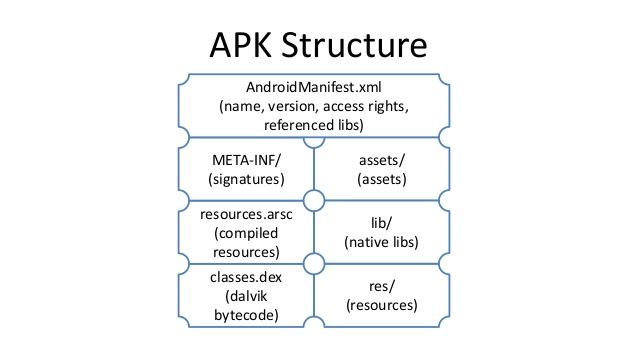
\includegraphics[width=10cm, height=10cm, keepaspectratio]{img/ApkStructure}\\[.5cm]
	
\end{figure}
\subsection{Conclusie APK-structuur}
Een APK bestaat dus uit 7 onderdelen. Deze onderdelen zullen echter wel verschillen van grootte. Indien de app veel afbeeldingen bevat zal de map res/ het grootste deel van de APK-grootte innemen. Indien de app veel code bevat zal het classes.dex bestand groter worden. In de proof-of-concept app, die later in deze studie wordt toegelicht, konden we volgende verhoudingen waarnemen tussen de groottes van de verschillende onderdelen: 
\begin{enumerate}
	\item classes.dex: 0.4\%
	\item res/: 98.3\%
	\item resources.arsc: 1.1\%
	\item AndroidManifest.xml: kleiner dan 0.01\%
	\item libs/: kleiner dan 0.01\%
	\item assets/: kleiner dan 0.01\%
	\item META-INF/: 0.2\% 
\end{enumerate}

\subsection{Verschillende app-profielen Android Wear}
Verder in deze studie zullen de verschillende compressietechnieken toegepast worden op een proof-of-concept app binnen elk van de 3 profielen (foto-apps, fitness-apps, CPU-intensieve apps). Hierdoor kan binnen elk app-profiel gekeken worden welke technieken het meeste invloed zullen hebben op de grootte van de APK. Ook zal voor elk app-profiel onderzocht worden of er al dan niet negatieve bijwerkingen zijn voor de prestaties van de app na compressie en hoe groot deze bijwerkingen zijn. Op deze manier kan dit onderzoek voor de ontwikkelaars van elk type app nagaan welke technieken voor hun app in ontwikkeling het meest effect zullen hebben op de grootte van de APK. Aan de hand van de resultaten van het onderzoek kan dan ook de afweging gemaakt worden of er voor hun applicatie niet te veel moet ingeboet worden op vlak van CPU- en geheugenprestaties van de app.

\subsubsection{Foto-apps}
Apps die veel gebruikmaken van foto's zullen in het algemeen vrij veel opslagruimte in beslag nemen, aangezien elke foto in de app meegeleverd wordt en de grootte van een foto snel kan oplopen tot 1MB. Indien de foto's niet meegeleverd worden in de APK van de app, dienen de foto's gedownload te worden van het internet en zal er dus meer netwerkactiviteit gebruikt worden en CPU verbruik om de foto te genereren op de juiste plaats in de app.
\subsubsection{GPS-intensieve apps}
Deze apps zullen de gebruiker vooral helpen bij het opvolgen van lichamelijke inspanningen en beweging. Bij deze apps wordt meestal gebruikgemaakt van de ingebouwde GPS in het Android Wear toestel. Doordat deze GPS constant actief is, zal het batterijgebruik van deze apps zeer hoog liggen.
\subsubsection{CPU-intensieve apps}
Apps die veel (visuele) informatie moeten genereren tijdens runtime, zullen in het algemeen een hoog CPU verbruik hebben. Een voorbeeld hiervan is een app die muziek afspeelt en intussen visuele effecten afbeeldt die gegenereerd worden op het tempo van de afgespeelde muziek.  

\section{Verschillende compressietechnieken}
\label{sec:compressietechnieken}

Uit de richtlijnen van Google voor het verkleinen van de grootte van de APK werden volgende technieken gekozen om te onderzoeken \autocite{googlereduceapksize}: 

\subsubsection{Gebruik Proguard en Dexguard}
Uit een interview met Cozmos, het bedrijf waarbij mijn co-promotor Joris Missiaen werkzaam is blijkt dat zij deze tools ook gebruiken : 
\begin{quote}
	\colorbox{lightgray}{\parbox{350px}{"De belangrijkste tool om de grootte van een APK te beperken is Proguard. Proguard zorgt er niet enkel voor dat je code moeilijker leesbaar wordt bij reverse engineering maar het verwijdert ook al je ongebruikte code en resources.
			Bij de grotere klanten waar ook security van groot belang is maken we gebruik van Dexguard. Dexguard is de commerciële variant van Proguard en gaat een stap verder met zijn compressietechnieken maar biedt daarnaast ook tal van andere features aan."
	}}
\end{quote}
Deze andere features zijn dan bijvoorbeeld bescherming tegen static analysis, beveiliging tegen klonen van de APK/SDK en bescherming tegen piraterij. Ook beschermt Dexguard tegen dynamic analysis (APK beveiligen tijdens runtime) door omgeving- en certificaatcontroles. 

\subsubsection{Verwijder ongebruikte resources}
\label{sec:removeunusedresources}
De ingebouwde lint tool in Android Studio, een statische code analyzer, detecteert resources in de res/ map die in de code niet gerefereerd worden. Android Studio zal hiervan een melding maken, maar zal deze niet automatisch verwijderen. Libraries die u toevoegt kunnen ongebruikte resources meebrengen. Gradle kan deze automatisch verwijderen als ``shrinkResources`` in de build.gradle wordt toegevoegd. 

\subsubsection{Verklein resource gebruik van libraries}
\label{sec:minimizeresourceslibraries}
Wanneer u een Android app ontwikkelt, worden vaak externe libraries gebruikt om de gebruiksvriendelijkheid te verhogen. Deze libraries bevatten vaak elementen die voor desktops of servers bedoeld zijn, deze elementen kunnen uit de libraries verwijderd worden indien de licentie dit toestaat. Deze techniek wordt ook gebruikt door Cozmos volgens Joris Missiaen: 
\begin{quote}
	\vspace{-15ex}
	\colorbox{lightgray}{\parbox{350px}{"Bij het gebruik van libraries kan het handig zijn om enkel de modules in je project te importeren die je ook daadwerkelijk nodig hebt. Ook kan het nuttig zijn om verschillende libraries tegenover elkaar af te wegen en te kijken welke de laagste method count hebben, het best met het geheugen omgaan, het minste plaats innemen, enz. Stel dat je een library aan je project zou willen toevoegen om images in te laden dan zou je de afweging kunnen maken tussen Glide en Picasso. Picasso is bijvoorbeeld 3,5 keer kleiner dan Glide, maar anderzijds gebruikt Glide een pak minder geheugen om een image weer te geven. Dat zijn afwegingen die je moet maken."}}
	\vspace{-3ex}
\end{quote}

\subsubsection{Ondersteun enkele specifieke schermdichtheden }
\label{sec:supportspecificdensities}
Vanaf Android 4.4 worden verschillende schermdichtheden ondersteund (ldpi, mdpi, tvdpi, hdpi, xhdpi, xxhdpi en xxxhdpi). Het is niet nodig om elke afbeelding te exporteren naar elke dichtheid. Android zal automatisch de afbeelding schalen naar andere schermdichtheden als er geen specifieke export voorzien is. 

\subsubsection{Verminder animatieframes }
\label{sec:reduceanimationframes}
Voor elke frame in een animatie wordt een aparte afbeelding opgeslagen. Als er bijvoorbeeld een animatie aanwezig is met 30 FPS (frames per second) zullen er 30 afbeeldingen opgeslagen worden, maar vaak is bijvoorbeeld 15 FPS meer dan voldoende. Op deze manier zijn er dus maar half zoveel animatieframes nodig.
\begin{figure}[H]
	\centering
	\caption{\textit{Door vermindering FPS zullen minder aparte afbeeldingen per animatie opgeslagen worden}\newline}
	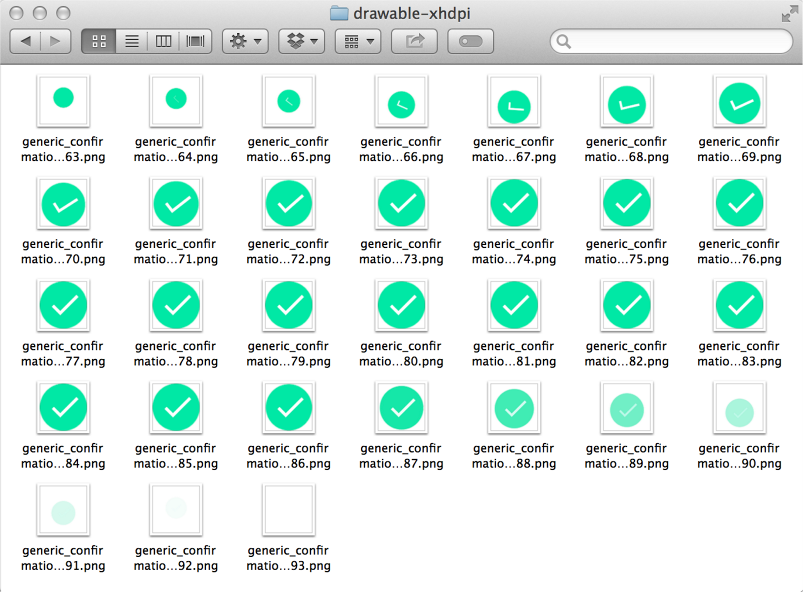
\includegraphics[width=10cm, height=10cm, keepaspectratio]{img/animation-frames}\\[.5cm]
	
\end{figure}
\subsubsection{Hergebruik resources }
\label{sec:reuseresources}
Het is mogelijk om voor elke variatie op een afbeelding (getint, met schaduw of geroteerd) een aparte resource op te slaan. Google raadt echter aan om één afbeelding te voorzien, en deze dynamisch tijdens runtime aan te passen. 
Android voorziet verschillende hulpprogramma's om de kleur van een afbeelding aan te passen.
\subsubsection{Comprimeer afbeeldingen }
\label{sec:compressimages}
De \cite{aapt} tool kan de afbeelding resources in res/drawable/ optimaliseren met lossless compressie. De tool kan bijvoorbeeld een true-color PNG bestand dat niet meer dan 256 kleuren bevat omzetten naar een 8-bit PNG met een kleurenpallet. Dit resulteert in een afbeelding van eenzelfde kwaliteit maar met een kleinere geheugenvoetafdruk. Deze tool kan geen PNG-bestanden in de asset/ folder verkleinen. Deze techniek wordt ook bij Cozmos gebruikt volgens Joris Missiaen: 
\begin{quote}
	\colorbox{lightgray}{\parbox{350px}{"Je kan al ruimte besparen door een juiste keuze te maken tussen JPG/PNG en verdere compressie toe te passen. Soms is ook geen volledige image nodig maar kan je opteren voor een 9-patch image of om een drawable in XML te definieren."}}
\end{quote}

\subsubsection{Gebruik WebP bestandformaat }
\label{sec:webp}
In plaats van PNG- of JPEG-bestanden, kan er ook gebruik gemaakt worden van het WebP formaat voor afbeeldingen. Dit formaat voorziet lossless compressie (zoals JPEG) en transparantie (zoals PNG) maar voorziet betere compressie dan beide andere formaten. Het gebruik van WebP heeft echter ook enkele nadelen. WebP-ondersteuning is niet beschikbaar bij versies lager dan Android 3.2 (API level 13). Het neemt ook een langere tijd voor het systeem om WebP bestanden te decoderen dan PNG bestanden. Bestaande BPM, JPG, PNG of statische GIF afbeeldingen kunnen naar het WebP formaat omgezet worden door Android Studio. 

\subsubsection{Gebruik vector graphics }
\label{sec:vectorgraphics}
Vector graphics kunnen gebruikt worden om resolutie-onafhankelijke iconen of andere schaalbare media te creëren. Deze afbeeldingen worden in Android gerepresenteerd als VectorDrawable objecten. Met een VectorDrawable object kan een 100-byte bestand een scherpe afbeeldingen genereren op de grootte van het scherm. 
Echter, het neemt een significante tijd voor het systeem om elk VectorDrawable object te genereren. Grote afbeeldingen kunnen zelfs nog meer tijd in beslag nemen om op het scherm te verschijnen. Daarom wordt aangeraden de VectorDrawable objecten enkel voor kleine afbeeldingen te gebruiken. 
\subsection{Verminder gebruik code}
\label{sec:reducecode}

\subsubsection{Verwijder automatisch gegenereerde code}
\label{sec:reducegeneratedcode}
Zorg dat u verstaat wat elke lijn gegenereerde code inhoudt en wat de voetafdruk ervan is. Zo zullen veel protocol buffer tools een groot aantal methodes en klassen genereren, die de grootte van de app kunnen verdubbelen of verdriedubbelen.

\subsubsection*{Verwijder enumeraties}
\label{sec:removeenumerations}
Elke enum kan 1 tot 1.4 KB grootte toevoegen aan uw app's classes.dex bestand. Deze toevoegingen kunnen snel oplopen voor complexe systemen of gedeelde libraries. Indien mogelijk gebruikt u best de @IntDef annotatie en ProGuard om enumeraties te strippen en om te zetten in integers. Deze conversie behoudt alle voordelen van enums. 
\subsubsection*{Verklein grootte native binaries}
\label{sec:reducesizenativebinaries}
Bij het gebruik van native code en de Android NDK (Native Development Kit, hierdoor kan je bepaalde delen van je app implementeren in native-code talen zoals C of C++) kan je de grootte van de app verkleinen door het optimaliseren van de code. Hiervoor zijn 2 technieken bruikbaar :
\begin{enumerate}
	\item \textbf{Debug symbolen verwijderen} \newline
	Wanneer de app niet meer in development is, zijn debug symbolen overbodig. Deze kan je uit de applicatie verwijderen door de ``arm-eabi-strip`` tool te gebruiken, deze zit ingebouwd  in Android NDK.
	\item \textbf{Vermijd het extraheren van native libraries} \newline
	Bewaar .so bestanden ongecompresseerd in de APK, en stel de ``android:extractNativeLibs`` vlag op false in het ``<application>`` element van je app manifest. Dit zal vermijden dat de PackageManager de .so bestanden uit de APK naar het bestandssysteem zal kopiëren tijdens de installatie, en zal als bijkomend voordeel hebben dat delta updates van de app kleiner zullen zijn. 
\end{enumerate}

\subsection{Voorzie meerdere APK's}
\label{sec:multipleapks}
De app kan inhoud bevatten die gebruikers downloaden maar nooit gebruiken, zoals regio- of taalgerelateerde informatie. Om een minimale download voor de gebruikers te voorzien, kan de app gesegmenteerd worden in verschillende APKs, gedifferentieerd door factoren zoals schermgrootte of GPU structuur.
Wanneer gebruikers de app downloaden zal hun toestel de correcte APK ontvangen gebaseerd op het toestel zijn instellingen en kenmerken. Op deze manier ontvangen hun toestellen geen inhoud bedoeld voor opties die het toestel niet heeft.


\section{Verband tussen compressie en prestaties apps}
\label{sec:verbandcompressieprestaties}
Bij Cozmos werd het volgende opgemerkt als verband tussen compressie en de prestaties van de apps :
\begin{quote}
	\colorbox{lightgray}{\parbox{350px}{"Er wordt zeker naar gekeken dat de performantie van de app goed zit. Bij het uitvoeren van network calls moet alles zo compact mogelijk zijn zodat een gebruiker ook onder een slechte verbinding kan blijven werken. Bij het tonen van meerdere afbeeldingen is het memory management zeer belangrijk om o.a. out of memory exceptions te vermijden. Op welk vlak de performantie een invloed heeft hangt af van ieder geval op zich. Je kan stellen dat er op één of meerdere van volgende punten verbetering merkbaar is": \begin{enumerate}
				\item \textbf{Grootte beperken}
				\item \textbf{Geheugen gebruik beperken}
				\item \textbf{Sneller laden}
			\end{enumerate}
	}}
\end{quote}


\section{Creatie proof-of-concept foto-app}
\label{sec:proofofconcept}

Om het onderzoek te onderbouwen, werd een Android Wear proof-of-concept app gecreëerd. Dit is een algemene applicatie, waarin verschillende elementen toegevoegd worden zoals media-bestanden en veel code. Het doel van de creatie van deze app is om de verschillende compressietechnieken hierop toe te passen en de resultaten grafisch voor te stellen. De applicatie draait op Android Wear 2.0. Deze versie werd op 09/02/2017 uitgebracht door Google \autocite{Google}. Doordat voor deze versie gekozen werd, kan de app als standalone app gebruikt worden. Dit houdt in dat de app op een smartwatch kan gebruikt worden onafhankelijk van een smartphone. De gebruikers kunnen meer taken, zoals muziek afspelen of foto's bekijken, op hun smartwatch uitvoeren zonder toegang tot een Android of iOS smartphone. De app zal als functie hebben om foto's weer te geven op de smartwatch, waar de gebruiker tussen kan wisselen door te tikken op het scherm. Op deze afbeeldingen werd vooraf nog geen compressie toegepast er werden afbeeldingen van een standaardgrootte gebruikt die dan automatisch geschaald werden naar de grootte van de image views. In de app zit ook een splashscreen verwerkt (scherm dat weergeven wordt tijdens het opstarten van de applicatie). Deze app zal dus als testapp gebruikt worden voor het app-profiel "Foto-apps". 
\begin{figure}[H]
	\centering
	\caption{\textit{Hoofdscherm foto-app}}
	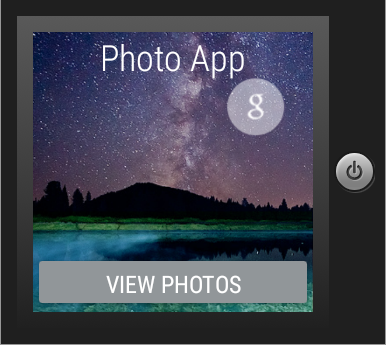
\includegraphics[width=7cm, height=7cm, keepaspectratio]{img/photoappmain}\\[.5cm]
\end{figure}
\begin{figure}[H]
	\centering
	\caption{\textit{Foto view}}
	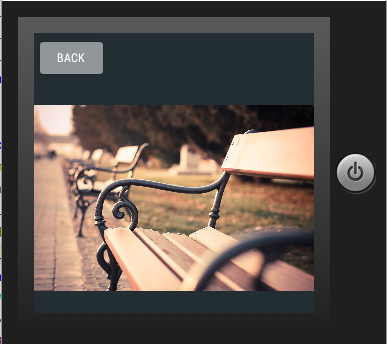
\includegraphics[width=7cm, height=7cm, keepaspectratio]{img/photoappgallery}\\[.5cm]
	
\end{figure}

%%=============================================================================
%% Literatuurstudie
%%=============================================================================


\chapter{Literatuurstudie}
\label{ch:literatuurstudie}

\section{Wat is Android Wear?}
\label{sec:androidwear}
Android Wear is Google's platform voor wearables. Een wearable worden beschreven door \textcite{Dictionary} beschreven als een computer of geavanceerd elektronisch toestel dat geïncorporeerd is in een accessoire gedragen op het lichaam of in een kledingstuk. 
\textcite{Techradar} heeft enkele van de belangrijkste kenmerken van Android Wear opgelijst.
Android Wear is gebouwd voor kleinere toestellen en met hands-free gebruik in het achterhoofd. Het maakt de toegang tot enkele van uw smartphone's makkelijkste functionaliteiten zo makkelijk als naar beneden kijken naar uw pols. Het is vooral bedoeld om de notificaties van uw smartphone makkelijk te weergeven zodat niet elke keer gezocht moet worden naar de smartphone in de broekzak. Gebaseerd op uw Google zoekopdrachten zullen real-time scores van uw favoriete sportteam, verkeerdscondities of afspraken in uw afgenda weergeven worden. Als het Android Wear toestel NFC (Near Field Communication) ingebouwd heeft, kan er in verschillende landen (momenteel Australië, Hong Kong, Ierland, Japan, Nieuw-Zeeland, Polen, Singapore, Verenigd Koninkrijk en de Verenigde Staten volgens de support van \cite{Androidpay}) ook met de wearable betaald worden via Android Pay. Ook spraakherkenning kon niet ontbreken in de Android Software. Door deze technologie kan je de wearable's spraakherkenning activeren door "OKay, Google" te zeggen of door de aanknop ingedrukt te houden. Google Assistant zal u hierop verderhelpen. Android Wear is compatibel met smartphones die draaien op Android 4.3 of hoger en iOS 9 of hoger. Eén van de belangrijkste app categorieën op Android Wear zijn de gezondheidsapps. Hiervoor wordt standaard gebruik gemaakt van Google Fit. Met Google Fit kan je kiezen tussen verschillende workouts tijdens het sporten, of bijvoorbeeld een dagelijks doel instellen voor het aantal stappen dat u wil nemen.  
\begin{figure}[h]
	\caption{Enkele voorbeelden van smartwatches gebruikmakend van Android Wear}
	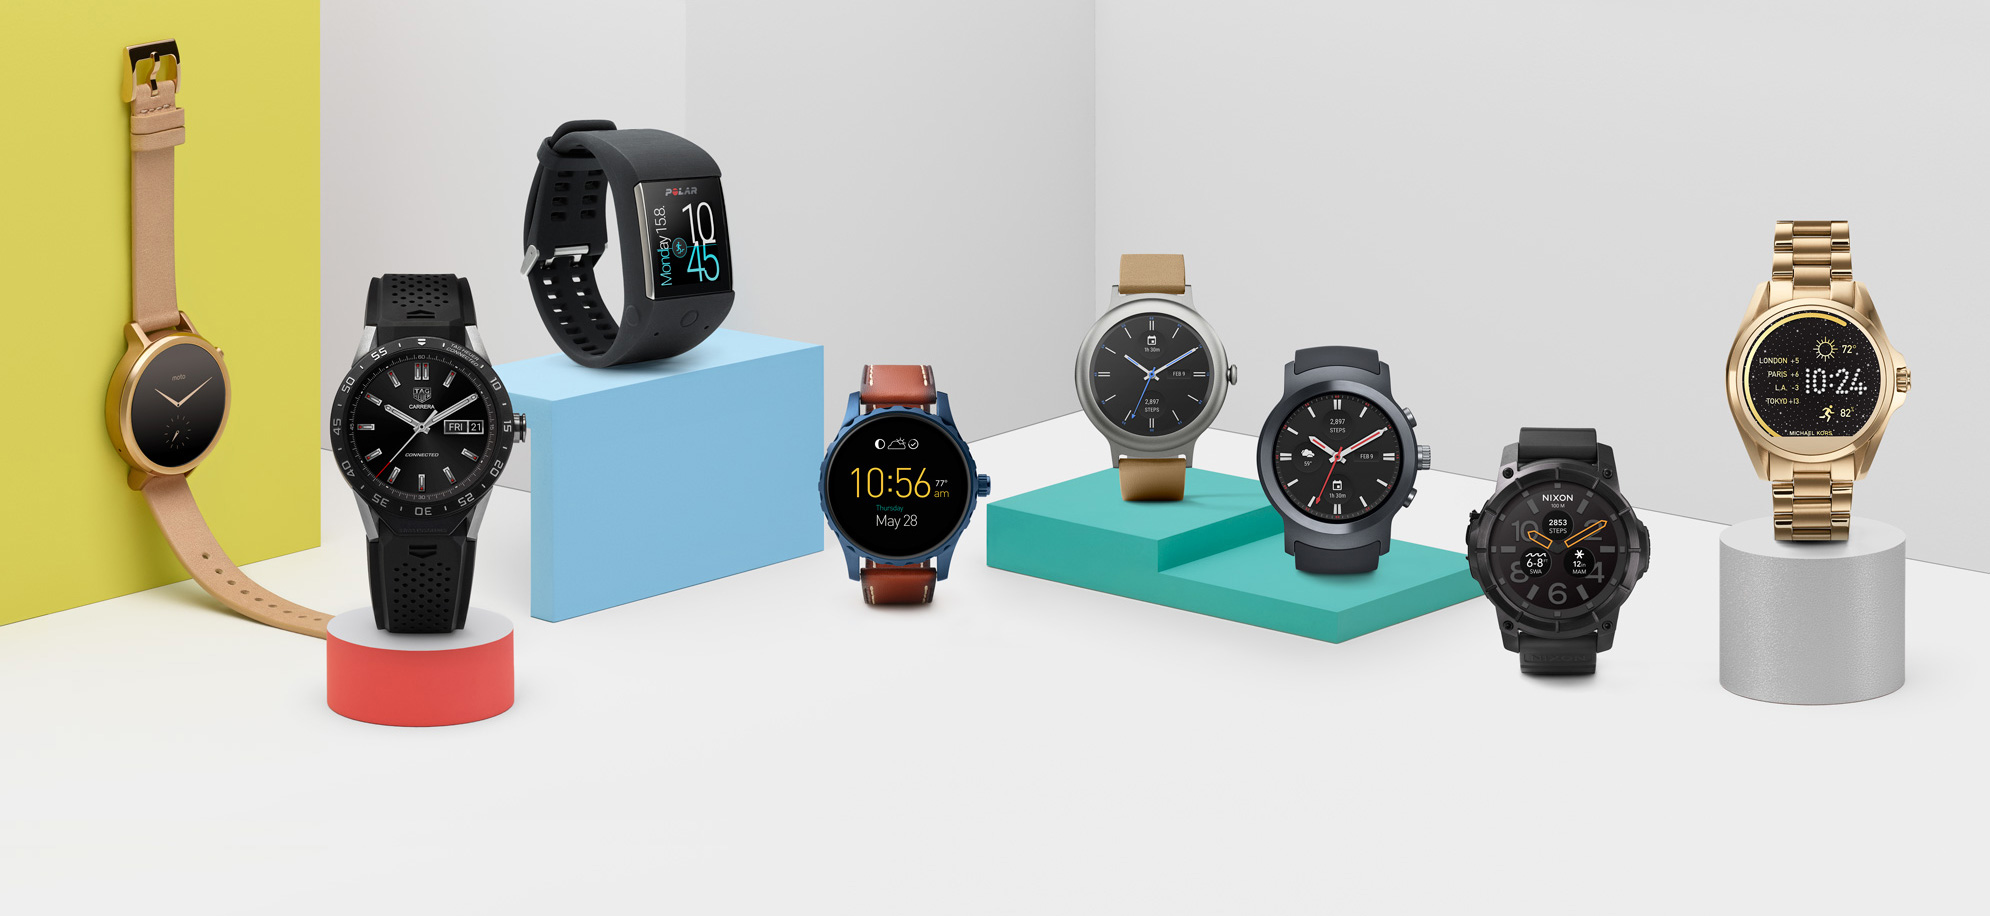
\includegraphics[width=15cm]{img/WearExamples}\\[.5cm]
	\centering
\end{figure}
%% TODO:
%% Uit je probleemstelling moet duidelijk zijn dat je onderzoek een meerwaarde
%% heeft voor een concrete doelgroep (bv. een bedrijf).
%%
%% Wees zo concreet mogelijk bij het formuleren van je
%% onderzoeksvra(a)g(en). Een onderzoeksvraag is trouwens iets waar nog
%% niemand op dit moment een antwoord heeft (voor zover je kan nagaan).
\section{Wat is een APK en uit wat bestaat dit?}
APK staat voor Android Application Package. Volgens \textcite{PCMag} is een APK een applicatie bestand klaar voor installatie op een Android toestel. Het gecompresseerde APK bestand, een ZIP archief in JAR-formaat, wordt gedistribueerd naar Android gebruikers voor de installatie op hun smartphone, tablet of wearable. 
Een APK bestand bestaat normaliter uit volgende elementen : 
\begin{enumerate}
	\setlength\itemsep{2em}
\item \textbf{classes.dex} \newline
Bevat gecompileerde applicatiecode, getransformeerd naar een Dex bytecode. Het is mogelijk dat er meerdere DEX bestanden in de APK staan als er multidex gebruikt wordt om de 65536 limiet te overkomen. Vanaf Android 5.0, met de introductie van ART runtime, worden deze bestanden gecompileerd naar OAT bestanden door de compiler bij de installatie en worden deze op het toestel zijn data partitie geplaatst. 
\item \textbf{res/} \newline
Deze folder bevat de meeste XML bestanden en drawables (bijvoorbeeld PNG of JPEG bestanden) in mappen met verschillende kwalificaties, zoals -mdpi en -hdpi voor schermdichtheden, -sw600dp of -large voor schermgroottes, en -en, -de, -pl voor talen. De XML bestanden worden automatisch gecompileerd naar een compactere binaire representatie, dus deze kunnen niet met een teksteditor geopend worden vanuit de APK. 
\item \textbf{resources.arsc}\newline
Sommige resources en identifiers worden gecompileerd naar dit bestand. Het wordt normaal ongecomprimeerd opgeslagen in de APK voor snellere toegang tijdens runtime. Dit bestand manueel comprimeren kan een makkelijke oplossing lijken, maar dit is geen goed idee door 2 redenen. Eén, Play Store comprimeert alle data voor transfer automatisch en twee, dit bestand comprimeren in de APK verspilt systeem resources (RAM) en performantie (vooral de opstarttijd van de app).
\item \textbf{AndroidManifest.xml}\newline
Gelijklopend met andere XML resources wordt de applicatie Manifest getransformeerd naar een binair formaat tijdens de compilatie. De Play Store gebruikt bepaalde informatie in de AndroidManifest om te bepalen of een APK kan geïnstalleerd worden op een bepaald toestel, zo zijn er controles op toegelaten schermdichtheden of schermgroottes, beschikbare hardware en kenmerken (bijvoorbeeld aanwezigheid van een touchscreen). Deze Manifest inhoud kan geïnspecteerd worden na compilatie, gebruik hiervoor de aapt tool van de Android SDK: 
\begin{lstlisting}[backgroundcolor = \color{lightgray}, xleftmargin = 2cm,
framexleftmargin = 1em]
$ aapt dump badging your_app.apk
\end{lstlisting}
\item \textbf{libs/}\newline
Alle native libraries (*.so bestanden) zullen in submappen geplaatst worden genaamd naar de ABI (CPU architectuur, bv. x86, \texttt{x86\_64}, armeabi-v7a) die ze als doel hebben onder de libs/ map. Normaal worden deze uit de APK gekopieerd naar de datapartitie tijdens het installeren van de applicatie. Echter, sinds de APK zelf nooit aangepast wordt zolang deze op het toestel van de gebruiker staat, neemt dit dubbel zoveel plaats in voor elke native library. 
\item \textbf{assets/}\newline
Deze map zal gebruikt worden voor alle bestandonderdelen die niet als Android-type resources gebruikt zullen worden. Meestal zullen dit lettertypebestanden of game data zijn, zoals levels of textures, samen met andere applicatiedata die direct geopend moet kunnen worden als een file stream.
\item \textbf{META-INF/}\newline
Deze map is aanwezig in ondertekende APKs en bevat een lijst van alle bestanden in de APK met hun handtekening. Momenteel werkt het ondertekenen van bestanden in Android door het verifiëren van de handtekening tegen de ongecomprimeerde bestandinhoud van het archief, één voor één. Dit heeft enkele interessante gevolgen. Doordat elke onderdeel van een ZIP bestand apart opgeslagen wordt, betekent dit dat je individuele bestanden hun compressieniveau kan aanpassen zonder ze opnieuw te ondertekenen. De verificatie van de handtekening zal echter falen wanneer een bestand verwijderd wordt uit het archief nadat het ondertekend werd. 
\end{enumerate}

\section{Verschillende compressietechnieken} \cite{googlereduceapksize}
\label{sec:compressietechnieken}

\subsection{Verklein resource aantal en grootte}
\label{sec:reduceresources}

\subsubsection{Verwijder ongebruikte resources}
\label{sec:removeunusedresources}
De ingebouwde lint tool in Android Studio, een statische code analyzer, detecteert resources in de res/ map die in de code niet gerefereerd worden. Android Studio zal hiervan een melding maken, maar zal deze niet automatisch verwijderen. Libraries die u toevoegt kunnen ongebruikte resources meebrengen. Gradle kan deze automatisch verwijderen als "shrinkResources" in de build.gradle wordt toegevoegd. 

\subsubsection{Verklein resource gebruik van libraries}
\label{sec:minimizeresourceslibraries}
Wanneer u een Android app ontwikkelt, worden vaak externe librbaries gebruikt om de gebruiksvriendelijkheid te verhogen. Deze libraries bevatten vaak elementen die voor desktops of servers bedoeld zijn, deze elementen kunnen uit de libraries verwijderd worden indien de licentie dit toestaat.

\subsubsection{Ondersteun enkele specifieke schermdichtheden }
\label{sec:supportspecificdensities}
Vanaf Android 4.4 worden verschillende schermdichtheden ondersteund (ldpi, mdpi, tvdpi, hdpi, xhdpi, xxhdpi en xxxhdpi). Het is niet nodig om elke afbeelding te exporteren naar elke dichtheid. Android zal automatisch de afbeelding schalen naar andere schermdichtheden als er geen specifieke export voorzien is. 

\subsubsection{Verminder animatie frames }
\label{sec:reduceanimationframes}
Voor elke frame in een animatie wordt een aparte afbeelding opgeslaan. Als er bijvoorbeeld een animatie aanwezig is met 30 FPS (frames per second) zullen er 30 afbeeldingen opgeslagen worden, maar vaak is bijvoorbeeld 15 FPS meer dan voldoende, en wordt dus de helft van de ingenomen opslagruimte gebruikt.

\subsubsection{Hergebruik resources }
\label{sec:reuseresources}
Het is mogelijk om voor elke variatie op een afbeelding (getint, met schaduw of geroteerd) een aparte resource op te slaan. Google raadt echter aan om 1 afbeelding te voorzien, en deze dynamisch tijdens runtime aan te passen. 
Android voorziet verschillende utiliteiten om de kleur van een afbeelding aan te passen.
\subsubsection{Comprimeer afbeeldingen }
\label{sec:compressimages}
De aapt tool kan de afbeelding resources in res/drawable/ optimaliseren met lossless compressie. De tool kan bijvoorbeeld een true-color PNG bestand dat niet meer dan 256 kleuren bevat omzetten naar een 8-bit PNG met een kleurenpallet. Dit resulteert in een afbeelding van eenzelfde kwaliteit maar met een kleinere geheugenvoetafdruk. Deze tool kan geen PNG bestanden in de asset/ folder verkleinen. 
\subsubsection{Gebruik WebP bestandformaat }
\label{sec:webp}
In plaats van PNG of JPEG bestanden, kan er ook gebruik gemaakt worden van het WebP formaat voor afbeeldingen. Dit formaat voorziet lossless compressie (zoals JPEG) en transparantie (zoals PNG) maar voorziet betere compressie dan beide andere formaten. Het gebruik van WebP heeft echter ook enkele nadelen. WebP-ondersteuning is niet beschikbaar bij versies lager dan Android 3.2 (API level 13). Het neemt ook een langere tijd voor het systeem om WebP bestanden te decoderen dan PNG bestanden. Bestaande BPM, JPG, PNG of statische GIF afbeeldingen kunnen naar het WebP formaat omgezet worden door Android Studio. 

\subsubsection{Gebruik vector graphics }
\label{sec:vectorgraphics}
Vector graphics kunnen gebruikt worden om resolutie-onafhankelijke iconen of andere schaalbare media te creëren. Deze afbeeldingen worden in Android gerepresenteerd als VectorDrawable objecten. Met een VectorDrawable object kan een 100-byte bestand een scherpe afbeeldingen genereren op de grootte van het scherm. 
Echter, het neemt a significante tijd voor het systeem om elk VectorDrawable object te genereren. Grote afbeeldingen kunnen zelfs nog langer nemen om op het scherm te verschijnen. Daarom wordt aangeraden de VectorDrawable objecten enkel voor kleine afbeeldingen te gebruiken. 
\subsection{Verminder gebruik code}
\label{sec:reducecode}

\subsubsection{Verwijder automatisch gegenereerde code}
\label{sec:reducegeneratedcode}
Zorg dat u verstaat wat elke lijn gegenereerde code inhoudt, en wat de voetafdruk ervan is. Zo zullen veel protocol buffer tools een groot aantal methodes en klassen genereren, die de grootte van de app kunnen verdubbelen of verdriedubbelen.

\subsubsection*{Verwijder enumeraties}
\label{sec:removeenumerations}
Elke enum kan 1 tot 1.4 KB grootte toevoegen aan uw app's classes.dex bestand. Deze toevoegingen kunnen snel oplopen voor complexe systemen of gedeelde libraries. Indien mogelijk gebruikt u best de @IntDef annotatie en ProGuard om enumeraties te strippen en om te zetten in integers. Deze conversie behoudt alle voordelen van enums. 
\subsubsection*{Verklein grootte native binaries}
\label{sec:reducesizenativebinaries}
Bij het gebruik van native code en de Android NDK (Native Development Kit, hierdoor kan je bepaalde delen van je app implementeren in native-code talen zoals C of C++) kan je de grootte van de app verkleinen door het optimaliseren van de code. Hiervoor zijn 2 technieken bruikbaar :
1) Debug symbolen verwijderen
Wanneer de app niet meer in development is, zijn debug symbolen overbodig. Deze kan je uit de applicatie verwijderen door de "arm-eabi-strip" tool te gebruiken, deze zit ingebakken in Android NDK.
2) Vermijd het extraheren van native libraries
Bewaar .so bestanden ongecompresseerd in de APK, and stel de "android:extractNativeLibs" vlag op false in het "<application>" element van je app manifest. Dit zal vermijden dat de PackageManager de .so bestanden uit de APK naar het bestandssysteem zal kopiëren tijdens de installatie, en zal als bijkomend voordeel hebben dat delta updates van de app kleiner zullen zijn. 
\subsection{Voorzie meerdere APK's}
\label{sec:multipleapks}
De app kan inhoud bevatten die gebruikers downloaden maar nooit gebruiken, zoals regio- of taalgerelateerde informatie. Om een minimale download voor de gebruikers te voorzien, kan de app gesegmenteerd worden in verschillende APKs, gedifferentieerd door factoren zoals schermgrootte of GPU structuur.
Wanneer gebruikers de app downloaden zal hun toestel de correcte APK ontvangen gebaseerd op het toestel zijn instellingen en kenmerken. Op deze manier ontvangen hun toestellen geen inhoud bedoeld voor opties die het toestel niet heeft.


\section{Verband tussen compressie en prestaties apps}
\label{sec:verbandcompressieprestaties}

%%=============================================================================
%% Resultaten
%%=============================================================================

\chapter{Resultaten}
\label{ch:resultaten}

\section{Vergelijking verschillende technieken}
\label{sec:technieken}

%% TODO:
%% Uit je probleemstelling moet duidelijk zijn dat je onderzoek een meerwaarde
%% heeft voor een concrete doelgroep (bv. een bedrijf).
%%
%% Wees zo concreet mogelijk bij het formuleren van je
%% onderzoeksvra(a)g(en). Een onderzoeksvraag is trouwens iets waar nog
%% niemand op dit moment een antwoord heeft (voor zover je kan nagaan).
Verschillende van de voorgestelde technieken worden reeds automatisch toegepast door Android Studio bij het compileren van de applicatie. Zo zit Proguard ingebouwd in Android Studio, worden ongebruikte resources verwijderd door de ingebouwde lint tool en kunnen enumeraties automatisch omgezet worden naar integers. Hierdoor zal het handmatig uitvoeren van deze technieken geen extra effect teweeg brengen. Daarnaast zal het effect van de technieken afhankelijk zijn van het app-profiel. 
Legende technieken : 
\begin{enumerate}
	\item Techniek0 = Geen compressietechniek toegepast
	\item Techniek1 = Verwijder ongebruikte resources
	\item Techniek2 = Comprimeer afbeeldingen
	\item Techniek3 = Gebruik WebP-formaat
	\item Techniek4 = Verklein grootte native binaries
\end{enumerate}
\subsection{Foto-app}
Bij de eerste applicatie die getest werd, een foto-app die veel mediabestanden bevat, had vooral het gebruik van het WebP-formaat voor alle afbeeldingen een grote invloed op de grootte van de APK. De andere technieken brachten op dit vlak geen verandering. Op vlak van het geheugengebruik van de applicatie tijdens runtime kon een minieme verandering opgemerkt worden na het toevoegen van de techniek ``Verklein resource gebruik van libraries``. Na de omzetting van de afbeeldingen naar het WebP-formaat verhoogde het CPU-gebruik met 9 procent. Dit wordt veroorzaakt doordat het genereren van de WebP-afbeeldingen meer CPU-kracht vergt.
\begin{figure}[H]
	\centering
	\caption{\textit{Resultaten verschillende compressietechnieken op APK-grootte foto-app}}
	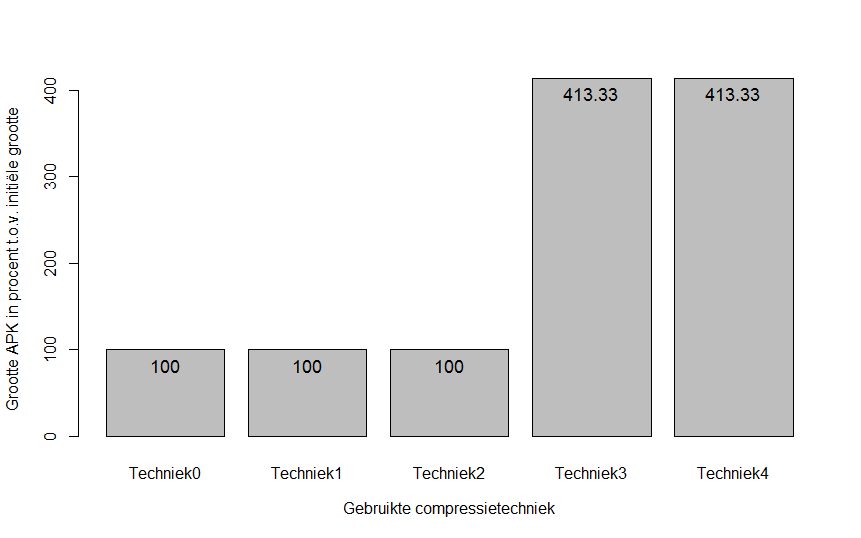
\includegraphics[width=10cm, height=10cm, keepaspectratio]{img/Rplot01}\\[.5cm]
	
\end{figure}

\subsection{Fitness-app}
\begin{figure}[H]
	\centering
	\caption{\textit{Resultaten verschillende compressietechnieken op APK-grootte fitness-app}}
	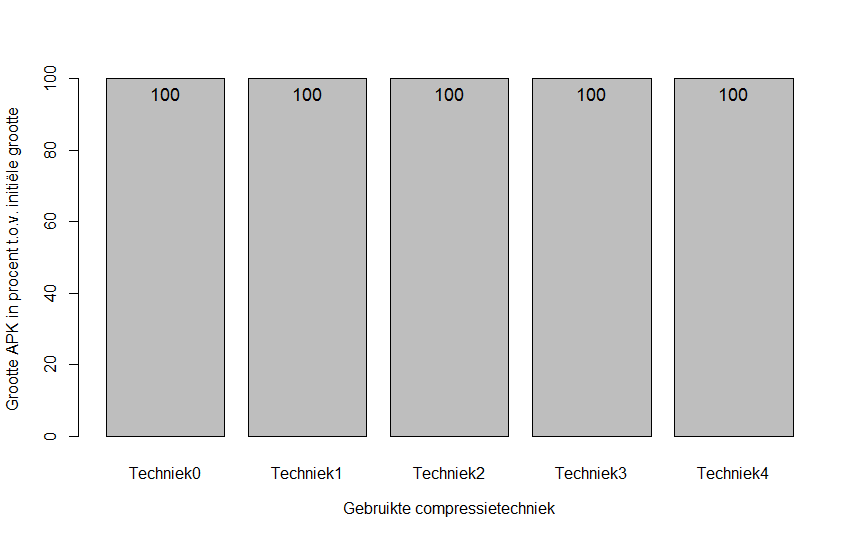
\includegraphics[width=10cm, height=10cm, keepaspectratio]{img/Rplot02}\\[.5cm]
	
\end{figure}
\subsection{CPU-intensieve app}
\begin{figure}[H]
	\centering
	\caption{\textit{Resultaten verschillende compressietechnieken op APK-grootte CPU-intensieve app}}
	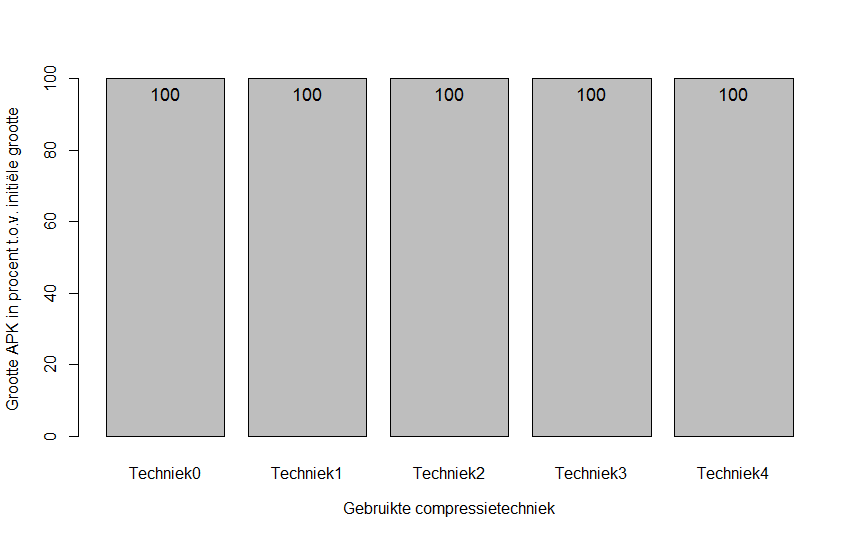
\includegraphics[width=10cm, height=10cm, keepaspectratio]{img/Rplot02}\\[.5cm]
	
\end{figure}

\section{Invloed compressie op prestaties apps}
\label{sec:invloedcompressie}
\subsection{Foto-app}
\subsubsection{Geheugengebruik}
\begin{figure}[H]
	\centering
	\caption{\textit{Resultaten verschillende compressietechnieken op geheugengebruik foto-app}}
	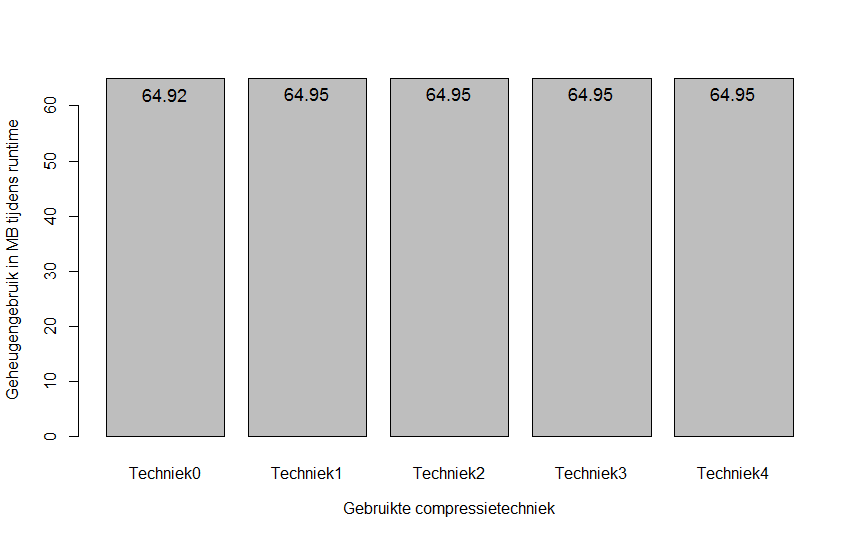
\includegraphics[width=10cm, height=10cm, keepaspectratio]{img/Rplot03}\\[.5cm]
	
\end{figure}
\subsubsection{CPU-gebruik}
\begin{figure}[H]
	\centering
	\caption{\textit{Resultaten verschillende compressietechnieken op CPU-gebruik foto-app}}
	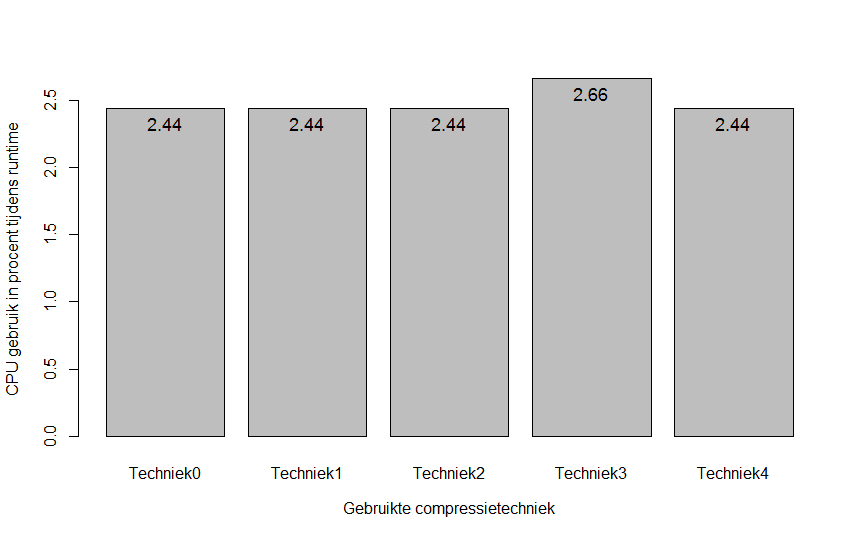
\includegraphics[width=10cm, height=10cm, keepaspectratio]{img/app1cpu}\\[.5cm]
	
\end{figure}
\subsection{Fitness-app}
\subsubsection{Geheugengebruik}
\begin{figure}[H]
	\centering
	\caption{\textit{Resultaten verschillende compressietechnieken op geheugengebruik fitness-app}}
	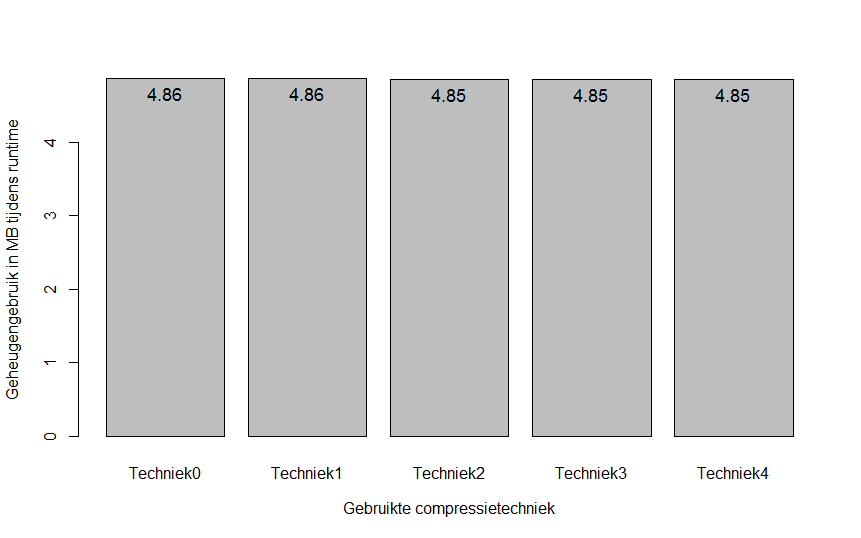
\includegraphics[width=10cm, height=10cm, keepaspectratio]{img/app2geheugen}\\[.5cm]
	
\end{figure}
\subsubsection{CPU-gebruik}
\begin{figure}[H]
	\centering
	\caption{\textit{Resultaten verschillende compressietechnieken op CPU-gebruik fitness-app}}
	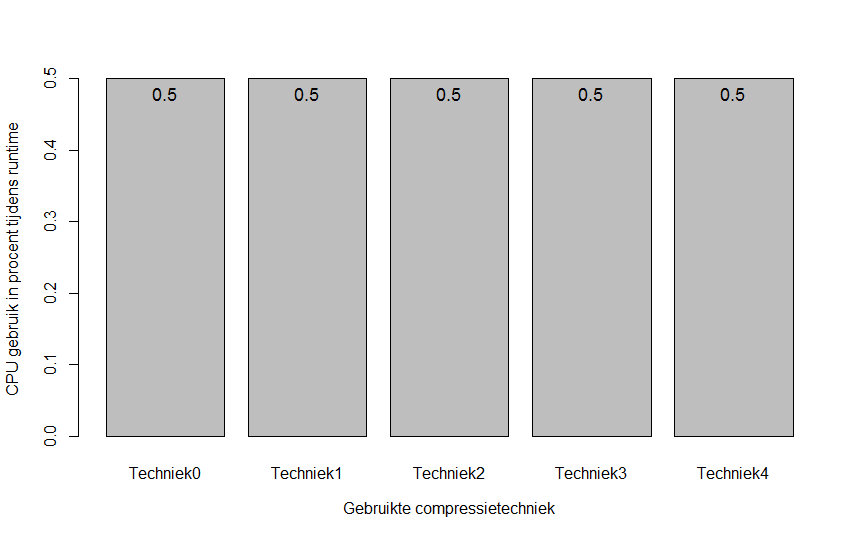
\includegraphics[width=10cm, height=10cm, keepaspectratio]{img/app2cpu}\\[.5cm]
	
\end{figure}
\subsection{CPU-intensieve app}
\subsubsection{Geheugengebruik}
\begin{figure}[H]
	\centering
	\caption{\textit{Resultaten verschillende compressietechnieken op geheugengebruik CPU-intensieve app}}
	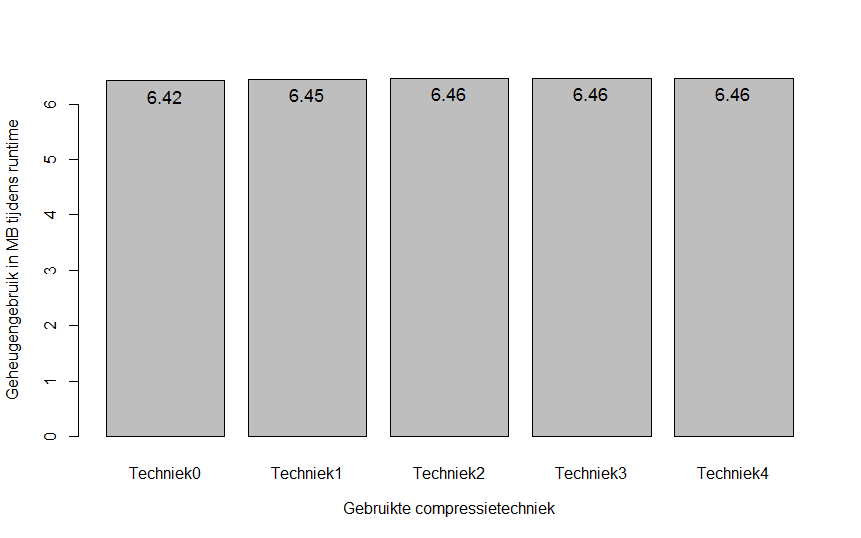
\includegraphics[width=10cm, height=10cm, keepaspectratio]{img/app3geheugen}\\[.5cm]
	
\end{figure}
\subsubsection{CPU-gebruik}
\begin{figure}[H]
	\centering
	\caption{\textit{Resultaten verschillende compressietechnieken op CPU-gebruik CPU-intensieve app}}
	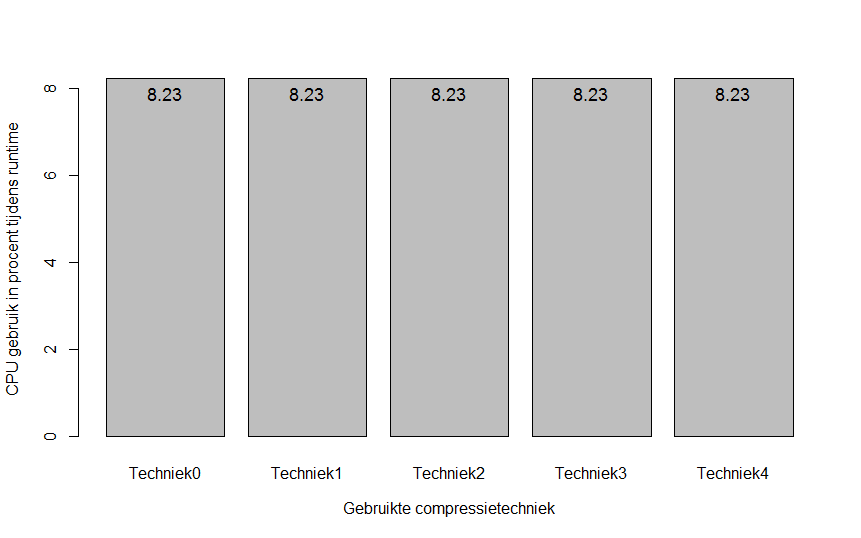
\includegraphics[width=10cm, height=10cm, keepaspectratio]{img/app3cpu}\\[.5cm]
	
\end{figure}

 \section{Testresultaten framework Brian Pinsard}
\label{sec:invloedcompressie}

%% Voeg hier je eigen hoofdstukken toe die de ``corpus'' van je bachelorproef
%% vormen. De structuur en titels hangen af van je eigen onderzoek. Je kan bv.
%% elke fase in je onderzoek in een apart hoofdstuk bespreken.

%\input{}
%\input{}
%...

%%=============================================================================
%% Conclusie
%%=============================================================================

\chapter{Conclusie}
\label{ch:conclusie}

%% TODO: Trek een duidelijke conclusie, in de vorm van een antwoord op de
%% onderzoeksvra(a)g(en). Wat was jouw bijdrage aan het onderzoeksdomein en
%% hoe biedt dit meerwaarde aan het vakgebied/doelgroep? Reflecteer kritisch
%% over het resultaat. Had je deze uitkomst verwacht? Zijn er zaken die nog
%% niet duidelijk zijn? Heeft het ondezoek geleid tot nieuwe vragen die
%% uitnodigen tot verder onderzoek?
\begin{appendices}
	\textbf{1. Worden bij Cozmos apps gecreëerd voor Android Wear? Zoja, zijn die dan standalone-apps of vooral apps die afhankelijk van de smartphone werken?}
	
	De projecten die we bij klanten doen starten tot nu toe altijd vanuit een gewone Android app. Klanten zoeken vaak een oplossing om hun interne processen te vereenvoudigen of ze willen aan hun klanten een app aanbieden.
	Door het grotere scherm, meer rekenkracht en simpelweg het feit dat bijna iedereen een smartphone bezit ligt de focus volledig daarop. Uiteraard hebben we al een aantal Android Wear projecten gehad maar dit was steeds ter aanvulling op een smartphone app. Voorbeelden hiervan zijn o.a. het tonen van je saldo op je watch of het slagen/falen van een transactie weergeven op je watch.
	
	\textbf{2. Welke compressietechnieken worden gebruikt bij Cozmos om de grootte van de APK zo klein mogelijk te houden?}
	
	De belangrijkste tool om de grootte van een APK te beperken is Proguard. Proguard zorgt er niet enkel voor dat je code moeilijker leesbaar wordt bij reverse engineering maar het verwijdert ook al je ongebruikte code en resources.
	Bij de grotere klanten waar ook security van groot belang is maken we gebruik van Dexguard. Dexguard is de commerciële variant van Proguard en gaat een stap verder met zijn compressietechnieken maar biedt daarnaast ook tal van andere features aan.
	
	Eén van de andere manieren om de grootte van je APK te gaan beperken is kijken naar de manier waarop je images en andere resources gaat gebruiken. Je kan al ruimte besparen door een juiste keuze te maken tussen jpg/png en verdere compressie toe te passen. Soms is ook geen volledige image nodig maar kan je opteren voor een 9-patch image of om een drawable in XML te definieren. Bij animaties kan je dan weer het aantal frames gaan beperken.
	
	Bij het gebruik van libraries kan het handig zijn om enkel de modules in je project te importeren die je ook daadwerkelijk nodig hebt. Ook kan het nuttig zijn om verschillende libraries tegenover elkaar af te wegen en te kijken welke de laagste method count hebben, het best met het geheugen omgaan, het minste plaats innemen, enz. Stel dat je een library aan je project zou willen toevoegen om images in te laden dan zou je de afweging kunnen maken tussen Glide en Picasso. Picasso is bijvoorbeeld 3,5 keer kleiner dan Glide maar anderzijds gebruikt Glide een pak minder geheugen om een image weer te geven. Dat zijn afwegingen die je moet maken.
	
	Een andere optie is om niet essentiële zaken achterwege te laten uit je APK. Afbeeldingen of data die maar voor een beperkte groep gebruikers van belang zijn kan je beter in realtime downloaden ipv. deze al in je APK te voorzien.
	
	Verder kan je ook door middel van je code zuiniger omspringen met storage. Zou dien je enums te vermijden, kan je (eenvoudige) images renderen, enzovoort. 
	
	Deze vraag kan natuurlijk vrij breed beantwoord worden. Er zijn waarschijnlijk nog wel andere dingen die ik nu over het hoofd zie maar ik denk dat bovenstaande al een goed beeld geeft. 
	
	\textbf{3. Wordt bij het gebruiken van compressietechnieken bij Cozmos ook gecontroleerd of deze compressie een effect heeft op de performantie van de app? Zoja, heeft u enig idee op welk vlak van performantie dit een invloed heeft en hoeveel dit een invloed heeft?}
	
	Er wordt zeker naar gekeken dat de performantie van de app goed zit. Bij het uitvoeren van network calls moet alles zo compact mogelijk zijn zodat een gebruiker ook onder een slechte verbinding kan blijven werken. Bij het tonen van meerdere afbeeldingen is het memory management zeer belangrijk om o.a. out of memory exceptions te vermijden. 
	
	Op welk vlak de performantie een invloed heeft hangt af van ieder geval op zich. Je kan stellen dat er op 1 of meerdere van volgende punten verbetering merkbaar is:
	\begin{enumerate}
		\item Grootte beperken
		\item Geheugen gebruik beperken
		\item Sneller laden
	\end{enumerate}
	
	Echt actief gaan monitoren welke prestatieverschillen een compressietechniek met zich meebrengt  daar hebben we meestal de tijd niet voor. Het is pas wanneer er bij het testen dingen naar boven komen dat er echt wordt gekeken welke extra stappen we kunnen ondernemen en welke winst er geboekt wordt. Uiteraard worden bovenstaande technieken tijdens het developen in het achterhoofd gehouden zodat er een optimaal resultaat bekomen wordt.
	
\end{appendices}




%%---------- Back matter ------------------------------------------------------

\printbibliography
\addcontentsline{toc}{chapter}{\textcolor{maincolor}{\IfLanguageName{dutch}{Bibliografie}{Bibliography}}}


\listoffigures
\listoftables

\end{document}
